% options:
% thesis=B bachelor's thesis
% thesis=M master's thesis
% czech thesis in Czech language
% slovak thesis in Slovak language
% english thesis in English language
% hidelinks remove colour boxes around hyperlinks

\documentclass[thesis=M,czech]{FITthesis}[2014/05/07]

\usepackage[utf8]{inputenc} % LaTeX source encoded as UTF-8

\usepackage[usenames,dvipsnames,svgnames,table]{xcolor}

\definecolor{lightgray}{rgb}{0.95, 0.95, 0.95}
\definecolor{darkgray}{rgb}{0.4, 0.4, 0.4}
\definecolor{purple}{rgb}{0.65, 0.12, 0.82}
\definecolor{editorGray}{rgb}{0.95, 0.95, 0.95}
\definecolor{editorOcher}{rgb}{1, 0.5, 0} % #FF7F00 -> rgb(239, 169, 0)
\definecolor{editorGreen}{rgb}{0, 0.5, 0} % #007C00 -> rgb(0, 124, 0)
\definecolor{orange}{rgb}{1,0.45,0.13}
\definecolor{olive}{rgb}{0.17,0.59,0.20}
\definecolor{brown}{rgb}{0.69,0.31,0.31}
\definecolor{purple}{rgb}{0.38,0.18,0.81}
\definecolor{lightblue}{rgb}{0.1,0.57,0.7}
\definecolor{lightred}{rgb}{1,0.4,0.5}

\definecolor{mygreen}{rgb}{0,0.6,0}
\definecolor{mygray}{rgb}{0.5,0.5,0.5}
\definecolor{mymauve}{rgb}{0.58,0,0.82}

\usepackage{courier}
%\usepackage{acronym}
\usepackage[printonlyused,withpage]{acronym}
%\usepackage[printonlyused,withpage]{acronym} \usepackage[printonlyused,withpage]{acronym} % ukaze jen pouzite zkratky, ukaze cislo stranky, kde byla zkratka poprve pouzita
\usepackage{enumitem}
\setlist{parsep=0pt,listparindent=\parindent}
\usepackage{listings}

\lstset{backgroundcolor=\color{lightgray},
keywordstyle=\color{blue},
stringstyle=\color{mymauve},
commentstyle=\color{mygreen},
morecomment=[l][\color{magenta}]{\#},
basicstyle=\footnotesize\ttfamily,
breaklines=true
}

\setcounter{secnumdepth}{5}

\usepackage{graphicx} %graphics files inclusion
% \usepackage{amsmath} %advanced maths
% \usepackage{amssymb} %additional math symbols

\usepackage{dirtree} %directory tree visualisation

\usepackage{nameref}

\setcounter{tocdepth}{2}

\usepackage{epigraph}
\setlength{\epigraphrule}{0pt}
\setlength{\epigraphwidth}{.95\textwidth}

% % list of acronyms
% \usepackage[acronym,nonumberlist,toc,numberedsection=autolabel]{glossaries}
% \iflanguage{czech}{\renewcommand*{\acronymname}{Seznam pou{\v z}it{\' y}ch zkratek}}{}
% \makeglossaries

\newcommand{\tg}{\mathop{\mathrm{tg}}} %cesky tangens
\newcommand{\cotg}{\mathop{\mathrm{cotg}}} %cesky cotangens

% % % % % % % % % % % % % % % % % % % % % % % % % % % % % % 
% ODTUD DAL VSE ZMENTE
% % % % % % % % % % % % % % % % % % % % % % % % % % % % % % 

\department{Katedra softwarového inženýrství}
\title{Adaptibilní systém pro doporučování obsahu}
\authorGN{Jan} %(křestní) jméno (jména) autora
\authorFN{Bouchner} %příjmení autora
\authorWithDegrees{Bc. Jan Bouchner} %jméno autora včetně současných akademických titulů
\supervisor{Ing. Jaroslav Kuchař}
\acknowledgements{Chci upřímně poděkovat všem, kteří mi věnovali čas, když jsem potřeboval pomoc při psaní této diplomové práce. Především vedoucímu práce Ing. Jaroslavu Kuchaři za správné směrování, celkový vhled do technologií a cenné rady. Děkuji také své rodině a všem přátelům za bezvýhradnou podporu během celých mých studií.}
\abstractCS{V~několika větách shrňte obsah a přínos této práce v~češtině. Po přečtení abstraktu by se čtenář měl mít čtenář dost informací pro rozhodnutí, zda chce Vaši práci číst.}
\abstractEN{Sem doplňte ekvivalent abstraktu Vaší práce v~angličtině.}
\placeForDeclarationOfAuthenticity{V~Praze}
\declarationOfAuthenticityOption{1} %volba Prohlášení (číslo 1-6)
\keywordsCS{Nahraďte seznamem klíčových slov v češtině oddělených čárkou.}
\keywordsEN{Nahraďte seznamem klíčových slov v angličtině oddělených čárkou.}

\begin{document}

% \newacronym{CVUT}{{\v C}VUT}{{\v C}esk{\' e} vysok{\' e} u{\v c}en{\' i} technick{\' e} v Praze}
% \newacronym{FIT}{FIT}{Fakulta informa{\v c}n{\' i}ch technologi{\' i}}

\begin{introduction}
	%sem napište úvod Vaší práce	
\begin{epigraphs}
\qitem{We are leaving the age of information and entering the age of recommendation.}%
 {---\textsc{Chris Anderson, 2004~\cite{anderson}}}
 \end{epigraphs}	
	Když se člověk před nástupem digitálního věku snažil mezi množstvím nabízených informací nalézt takové, které by pro něj byly nějakým způsobem užitečné, musel se často spíše než na vlastní úsudek spoléhat na doporučení svých známých a přátel nebo na obecnou oblibu. Tu ale více než cokoliv jiného určoval aktuální společenský trend. Tato situace úzce souvisela s nedostatečným množstvím dat.

	S rozvojem internetu začalo narůstat i množství dostupných informací\footnote{Organizace IDC došla v článku~\emph{Extracting Value from Chaos} k závěru, že objem světových dat se každé dva roky zdvojnásobuje.~\cite{digitaluniverse}}. Nová data jsou produkována takřka každou sekundu, což vede k opačnému extrému – k jejich setřídění nám nyní nezbývá čas. Ceněným uměním je tak schopnost vytěžit maximum užitečných informací a ty posléze využít k nabytí nových znalostí.
	
	K těmto účelům přispěl velkou měrou rozvoj disciplíny zvané jako informační filtrování, čímž je myšlenka selekce a redukce informací. Odtud už je jen krok k personalizovanému doporučování obsahu, které se v posledních několika letech rozmáhá se zaváděním \emph{doporučovacích systémů}. 

	Hned na začátku práce jsem si dovolil citovat bývalého šéfredaktora časopisu Wired Chrise Andersona (článek \emph{The Long Tail~\cite{anderson}}, který shrnul nastalou situaci týkající se vývoje informací do jedné stručné věty. Je důležité vzít v potaz, že Anderson toto prohlášení učinil v roce 2004. 
	
	Vývoj v oblasti informačních technologií je neúprosný a každý další rok je ve znamení výrazných pokroků ve vývoji všech oborů, těch zaměřených na doporučování nevyjímaje. Od vstupu do \emph{doporučovací éry} uplynulo deset let a situace je nyní taková, že s pouhou znalostí ověřených doporučovacích algoritmů lze sice ještě stále dosáhnout měřitelných úspěchů (například nasazením některého z doporučovacích algoritmů do programové logiky menšího e-shopu), pro globálnější potřeby je to však již poněkud málo.
	
	Tajemstvím úspěšných systémů, jakými disponují například společnosti Google či Amazon, je aplikovaný výzkum a vývoj opírající se nejčastěji o teorii pravděpodobnosti a statistiky, strojového učení a dalších oblastí umělé inteligence.

	Budoucnost je tedy v systémech, které dokáží sestavovat svá doporučení na základě pokročilejší analýzy, a které jsou schopny přizpůsobit svá doporučení uživatelům na míru.
	
	Jedním takovým přístupem je kombinování více doporučovacích metod dohromady a sestavování výsledků na základě zaznamenávaného vývoje.

\section{Motivace} 	
\label{sec:motivation}
	Představme si nyní podobný systém jako rádce, který je schopen v každém okamžiku rozhodnout, co je pro uživatele, kteří žádají systém o radu, nejvhodnější. Rádce těmto uživatelům sděluje informace o typu doporučení (doporučovacím algoritmu), jehož použití by v \emph{danou chvíli} mohlo vést k maximalizaci užitku z doporučeného obsahu.
	
	Za \emph{danou chvíli} je považována kombinace několika vstupních proměnných, například denní doba, zařízení, ze kterého je žádáno o obsah, den v týdnu či geografická lokace uživatele.
	
	Pokud bude uživatel dbát rádcových rad, s největší pravděpodobností obdrží doporučení, se kterým bude spokojen, a svou spokojenost vyjádří například tím, že u jedné z doporučených položek zažádá o bližší detaily nebo ji nějakým dalším způsobem ohodnotí. 
	
	Jinými slovy, uživatel zašle rádci zpětnou vazbu týkající se toho, jak kvalitní bylo dané doporučení.
	
	Rádce sám neprovádí žádné operace, dokud k nim není explicitně vyzván. V paměti si uchovává pouze vnitřní stav, na základě kterého rozhoduje o doporučeních. Díky průběžné analýze a přepočítávání zpětné vazby je schopen pružně reagovat na situace, kdy dojde k náhlé a hromadnější změně preferencí nebo vyvstanou jiné události, jež by měly za následek dlouhodobější doporučování nevhodného obsahu.
	
\section{Cíle práce}
\label{sec:objectives}
	Nejdůležitějším cílem této práce je návrh a implementace rádce, neboli adaptibilního systému, který by byl schopen automaticky a vhodně kombinovat metody pro doporučování obsahu, rozdávat rady a přizpůsobovat se podmínkám. Součástí práce je také výběr a implementace vhodné sady algoritmů, které budou použity pro kombinování.

	Vzniklý systém bude schopen zpracovávat zpětnou vazbu od uživatelů týkající se kvality jimi zvoleného doporučení. Zpětná vazba by měla fungovat na principu odměny za dobré doporučení či trestu za špatné, což povede k ovlivňování preferencí při kombinování v čase.
		
	Nezbytnou součástí diplomové práce je osvojení základních pojmů a pravidel z oblasti strojového učení, teorie pravděpodobnosti a statistiky. Těchto znalostí je využíváno zejména v části práce týkající se predikce vhodného algoritmu a dopadu zpětné vazby na vývoj systému. 
	
	Vzhledem k povaze projektu je nutné navrhnout obecné rozhraní jak pro manipulaci s doporučovacími algoritmy, tak pro adaptibilní systém a jeho součásti.
	
	Funkčnost vyvinutého řešení bude na závěr ověřena implementací modelové úlohy simulující interakci více uživatelů s adaptibilním systémem. 
	
	K dosažení těchto cílů bude zapotřebí navrhnout a vyvinout následující části:

\begin{itemize}
  \item \textbf{Adaptibilní systém pro doporučování obsahu.}
  \item \textbf{Sada základních algoritmů určených k doporučování.}
  \item \textbf{RESTful API pro manipulaci s doporučovacími algoritmy a systémem.}
  \item \textbf{Klientská aplikace pro simulaci modelové úlohy.}  
\end{itemize}	

\section{Struktura práce}
\label{sec:structure}
	Tato práce je strukturována do 3 různých kapitol. Kapitoly jsou řazeny v pořadí, v jakém probíhaly jednotlivé fáze vývoje.	

\begin{description}
  \item[Kapitola \nameref{chap:teor}] Popisuje trendy používané současnými doporučovacími systémy a zkoumá algoritmické a matematické postupy, které by mohly být použity při návrhu strategie adaptibilního systému.
  \item[Kapitola \nameref{chap:prakt}] Shromažďuje veškeré požadavky kladené na systém, dále se zabývá návrhem architektury, detailními návrhy serverové i klientské části, rozhraním zastřešujícím komunikaci těchto částí a výběrem základní sady algoritmů, které budou využity k doporučování obsahu. Popisuje též postupy užité při vývoji aplikace na základě provedené analýzy a návrhu.
  \item[Kapitola \nameref{chap:tests}] Shrnuje poznatky nabyté z prováděných experimentů se systémem a stanovuje pravidla pro nejlepší použití.
  \item[Kapitola \nameref{chap:futurework}] Hodnotí vzniklou aplikaci a zamýšlí se nad dalším kroky ve vývoji aplikace.
\end{description}
	
\end{introduction}

\chapter{Teoretická část}		
\label{chap:teor}

\section{Doporučování obsahu}	
\label{chap:current}

Všechna doporučení sdílejí stejnou myšlenku – zaujmout či upozornit na něco konkrétního, co by pro nás jako uživatele mohlo být nějakým způsobem zajímavé. Spousta elektronických obchodů, renomovaných aukčních domů, ale též serverů se zábavou na doporučování doslova staví své podnikání.

\subsection{Analýza vybraných systémů}
\label{sec:examples}
Na internetu lze narazit na desítky, ba i stovky systémů zapojených do reálného provozu. Záměrně jsem se snažil vybral pouze zlomek, jenž by ale zároveň pokrýval většinu typů doporučovaného obsahu (produkty, články, zábava apod.).

U těchto systémů jsem se snažil identifikovat, jaké postupy jsou prováděny na pozadí jejich doporučování a jaké k tomu využívají metody. Vzhledem k povaze řešeného problému jsem zkoumal též znaky týkající se kombinování metod, kterými bych se mohl nechat inspirovat při návrhu svého systému.

\subsubsection{Amazon.com}

\textbf{Amazon.com, Inc.}\footnote{\url{http://www.amazon.com}} je jedním z největších a nejstarších internetových prodejců. Společnost začínala jako online knihkupectví, postupem let však zařadila do své prodejní nabídky též hudební a filmové nosiče, software, elektroniku, nábytek a spoustu dalšího zboží včetně vlastní spotřební elektroniky v podobě čtečky elektronických knih a tabletů Kindle či poskytování služeb z oblasti cloud computingu.

Firmu lze řadit mezi průkopníky doporučování na internetu. Jako jeden z prvních internetových prodejců začala svým zákazníkům doporučovat výrobky na základě nákupů jiných uživatelů.

Doporučovací systém společnosti je založen na více zdrojích informací:

\begin{itemize}
	\item Porovnávání uživatelem prohlížených položek a položek umístěných uvnitř nákupního košíku s položkami, které se společně s těmito prohlíženými položkami v minulosti často prodávaly\footnote{affinity analysis – nacházení spojení mezi odlišnými položkami. Základním příkladem budiž vztah mezi šamponem a kondicionérem. Kupující je většinou používá v ten samý čas~\cite{affinity}. Při nákupu jednoho by mohl mít tedy zájem i o druhý.}.
	\item Uchovávání informací ohledně hodnocení položek uživateli.
	\item Zaznamenávání nákupní historie.
	\item Sledování spousty dalších postupů, jako například vyhodnocování demografických informací (dle doručovací adresy), zaznamenávání pohybu po stránce (jaké všechny položky si uživatel prohlédl, než vložil jednu konkrétní do nákupního košíku) nebo sledování prokliků\footnote{Jako proklik se označuje takové kliknutí na odkaz, které uživatele dovede na cílovou stránku~\cite{proklik}.} z marketingových e-mailů s odkazy na zboží~\cite{amazonrec} a jejich vzájemná kombinace.
\end{itemize}

Kromě výše uvedeného využívá společnost strategii \emph{item-to-item kolaborativní filtrování}.

Díky vzájemné kombinaci všech těchto pravidel a metod nalezne fanoušek moderních technologií při návštěvě stránek především odkazy na technologické novinky všeho druhu, zatímco mladá matka bude mít v nabídce té samé stránky ve větší míře zastoupeno dětské zboží.
 
Výše jsou samozřejmě popsány pouze základní principy. Doporučovací systém společnosti jako takový je velmi komplexní a detaily algoritmu jsou drženy jako obchodní tajemství. K nahlédnutí jsou ale patenty, např. \emph{Personalized recommendations of items represented within a database}~\cite{jacobi2006personalized} nebo \emph{Collaborative recommendations using item-to-item similarity mappings}~\cite{linden2001collaborative}.

\subsubsection{Netflix}

\textbf{Netflix, Inc.}\footnote{\url{https://www.netflix.com}} je společnost, poskytující v začátcích své služby jako internetová videopůjčovna, jež se v průběhu posledních několika let rozrostla v obrovskou mediální společnost. Strategicky významným byl pro ni rok 2007. Tehdy byla nabídka jejích služeb rozšířena o filmy přenášené přes stream\footnote{Snímek se fyzicky nenachází na koncovém zařízení, ale přehrává se přímo ze serveru poskytovatele .}~\cite{netflix2007}. Nyní společnost nabízí obsah v podobě filmů a seriálů pro většinu v dnešní době používaných platforem jako PC, Mac, PlayStation3, Wii, Xbox a také pro mobilní telefony a tablety. 

Vzhledem k tomu, že firma staví své podnikání na tom, že její zákazníci ji platí za konzumaci zábavy, je v jejím vlastním zájmu, aby těmto uživatelům sledujícím filmy a seriály nabízela automaticky další obsahově či žánrově podobné, zkrátka takové, jenž budou co možná nejvíce lahodit jejich vkusu (dle~\cite{netflixrec} pochází $\frac{2}{3}$ zapůjčených filmů na Netflix z předchozího doporučení). Úspěšné podnikání společnosti je tak přímo závislé na tom, jak kvalitním doporučovacím systém společnost disponuje. 

\paragraph{Netflix Prize}
Za tímto účelem vyvinula společnost vlastní systém \emph{Cinematch} napomáhající svým zákazníkům objevit pro ně zajímavé filmy. Postupný vývoj na poli doporučovacích systémů však přivedl společnost na otázku, zda není možné vyvinout systém, jenž by dokázal Cinematch v oblasti předpovídání filmového vkusu porazit.Společnost tak vypsala začátkem října 2006 soutěž známou jako \emph{Netflix Prize}. Týmu, kterému by se podařilo zlepšit dosavadní výsledky systému Cinematch alespoň o 10 procent, by byla přiřknuta odměna ve výši 1 milion amerických dolarů.

Do soutěže byla uvolněna sada testovacích dat obsahující:

\begin{itemize}
	\item ID uživatele
	\item ID filmu
	\item hodnocení na intervalu $\langle1,5\rangle$
	\item datum uskutečnění hodnocení
\end{itemize}

Data obsahovala 100 480 507 takových hodnocení pro 17 770 filmů od 480 189 uživatelů. Uvolněna byla ještě další sada testovacích dat obsahující stejné informace, jen s vynecháním uživatelských hodnocení. Cílem pak bylo predikovat tato chybějící hodnocení opět na intervalu $\langle1,5\rangle$~\cite{netflixrules}.

Celková výhra byla udělena až v roce 2009 (do té doby sice docházelo k průběžnému zlepšování výsledků, nikdy však nebylo dosaženo požadovaného zlepšení 10 procent) týmu \emph{BellKor's Pragmatic Chaos}, vzniklého spojením tří do té doby samostatně soutěžících týmů.

Vítězný tým dosáhl cíle pomocí \emph{pokročilých technik strojového učení}. Zjistil přitom především to, že hodnocení každého filmu je silně subjektivní záležitostí, kterou je velmi obtížné programově předpovědět. Ukázalo se také, že ve větší míře záleží na tom, zda uživatel hodnotí právě dosledovaný film nebo film, který zhlédl již před delší dobou. Velkou roli hraje i nálada uživatele v průběhu dne, zda film sleduje například o víkendu, kdy má volno a tak podobně~\cite{bellkor}.

Výsledný algoritmus, jenž získal cenu, vznikl kombinováním zhruba stovky menších algoritmů. S trochou nadsázky lze tedy prohlásit, že jednou z hlavních taktik pro kvalitní doporučení je \emph{použití tolika algoritmů, kolik je jen možné}.

\subsubsection{Mendeley}	
\label{mendeley}
\textbf{Mendeley}\footnote{\url{http://www.mendeley.com}} je systém určený k doporučování vědeckých článků využívající jako svou výpočetní vrstvu technologii Apache Mahout\footnote{https://mahout.apache.org}. Cílem systému je spojovat dohromady výzkumníky a jejich data. Svým uživatelům napomáhá v organizaci výzkumu, umožňuje jim navázat potenciální spolupráci s dalšími uživateli aplikace a napomáhá též k objevení nových podnětů pro vlastní práci. Uživateli této aplikace jsou přední světové university jako University of Cambridge, Stanford University, MIT či University of Michigan. Data pro aplikaci pocházejí z vlastních importů uživateli i z externích importů skrze různé katalogy vědeckých prací. 

Projekt samotný se v jedné ze svých prezentací~\cite{mendeleylastfm} přirovnává k největší hudební databázi na internetu – last.fm\footnote{http://www.last.fm}. Ta funguje na principu, že potenciální uživatel provede na svém počítači instalaci desktopové aplikace, následně s již instalovanou aplikací začne poslouchat hudbu a tím je zahájeno automatické odesílání informace o skladbě (interpret, žánr) na server last.fm. Podle dat odeslaných na server jsou uživateli v budoucnu doporučovány další skladby. 

Mendeley tuto analogii vysvětluje tak, že hudební knihovny jsou v jeho případě výzkumné knihovny, role interpretů zastávají jednotliví výzkumníci, hudební skladby jsou pak jimi publikované články a jednotlivé hudební žánry reprezentují vědecké disciplíny.  

Doporučení jsou dle dostupných informací~\cite{mendeleylastfm} generována dvojím způsobem. 

\begin{description}
	\item[Kolaborativní filtrování] Používá se pro personalizované doporučení. Podporována je jak user-based, tak item-based varianta.
	\item[Filtrování založené na obsahu] Používá se k nalezení souvisejících výzkumů, například pro nalezení článku ze stejné výzkumné kategorie nebo článku majícího podobný název. 
\end{description}

Uživatelé vyjadřují svůj zájem či nezájem o každou z doporučených položek zpětnou vazbou, která je dvojího typu:

\begin{description}
	\item[Accept] vyjadřuje, že uživatel s daným doporučením souhlasí nebo pro něj bylo nějakým způsobem užitečné.
	\item[Remove] vyjadřuje nevhodné doporučení. Uživatel touto volbou dává najevo, že podobné doporučení by příště již raději nedostal.
\end{description}

\subsubsection{Google News}	

Vlastní platformu pro doporučování obsahu vytvořila v rámci svého vývoje též společnost \textbf{Google, Inc.}~\footnote{\url{http://www.google.com/about/company}}. Její výzkumníci se v práci~\cite{googlenews} zabývali vývojem prediktivního systému pro personalizované doporučování zpráv na webu Google News~\footnote{\url{http://news.google.com}}.

Přihlášeným uživatelům, majících v prohlížeči explicitně povolen záznam historie prohlížení, jsou generována doporučení založená na zájmu těchto uživatelů, která vycházejí z různých profilů sestavených pozorováním chování uživatelů na stránce.  

K porozumění, jak se mění zájem uživatelů o zprávy v čase, napomohla výzkumníkům analýza logů (záznamy chování anonymních uživatelů na stránce). Na základě této analýzy byl vyvinut Bayesovský framework pro předvídání zájmu uživatelů o zveřejňované novinky.

Kombinace mechanismu pro filtraci informací vzešlého z nashromážděných uživatelských profilů a již existujícího mechanismu využívajícího principů kolaborativního filtrování vedla ke vzniku systému generujícího personalisované zprávy. Vzniklá kombinace byla nasazena do reálného provozu a následné experimenty prokázaly, že kombinováním metod došlo ke zlepšení kvality doporučování.

\subsubsection{Výzkum}

Také současný výzkum v oblasti doporučovacích systémů, zdá se, nezahálí. Zde uvádím příklad dvou populárních akcí, jejichž náplní či součástí je problematika doporučování a doporučovacích systémů.

\begin{itemize}
  \item \textbf{ACM RecSys conference.}~\footnote{\url{http://recsys.acm.org}} Konference je předním mezinárodním fórem pro prezentaci nových výsledků výzkumu a postupů na poli doporučovacích systémů. RecSys sdružuje hlavní mezinárodní výzkumné skupiny a též mnoho předních světových společností na trhu e-commerce. Nabízí také doprovodný program v podobě zvaných přednášek, konzultace týkající se problematiky RecSys a sympózium studentů doktorských programů. 
  
  Zajímavé prezentace jsou volně dostupné na internetu, dá se tedy načerpat spousta inspirace do vlastního výzkumu. Mě osobně velmi zaujala prezentace~\footnote{\url{http://www.slideshare.net/d0nut/open-recommendation-platform}} z posledního ročníku konference (Hong Kong, 2013), se kterou vystoupil Torben Brodt, jeden z klíčových řečníků. V prezentaci popisuje tzv. \emph{Open Recommendation Platform}~\ref{sub:orp}. 
  
  \item \textbf{ICWSM: Weblog and Social Media.}~\footnote{\url{http://www.icwsm.org/2014}} The International AAAI Conference on Weblogs and Social Media je mezinárodní konference, na které se střetávají výzkumní pracovníci z oblasti počítačových a společenských věd. Konference je pořádaná za účelem sdílení znalostí, diskutování o nápadech a výměny informací. Probíranými body jsou psychologické a sociální teorie, výpočetní algoritmy pro analýzu sociálních médií a jedním z mnoha témat jsou též doporučovací systémy.
\end{itemize}

O tématu se též píše spousta článků a každým rokem vzniká několik disertačních prací. Dle dostupných informací z ACM RecSys Wiki~\footnote{\url{http://www.recsyswiki.com/wiki/List_of_recommender_system_dissertations}} jich jen za poslední 4 roky bylo přes 50.

\subsubsection{Open Recommendation Platform}
\label{sub:orp}
\textbf{Open recommendation Platorm} (zkr. ORP) je projekt společnosti \textbf{plista}\footnote{\url{https://www.plista.com}} prezentovaný na posledním ročníku konference ACM RecSys 2013 v Hong Kongu. 

Motivací ORP bylo dosáhnout lepších výsledků kombinací více metod doporučování obsahu společně se zapojením kontextu uživatele (informacemi čerpanými převážně z HTTP hlaviček). Informacemi, které využívají, jsou například:

\begin{itemize}
	\item IP adresa, která může prozradit geologickou lokaci uživatele,
	\item denní doba, kdy uživatel přistupuje ke stránce,
	\item user agent prohlížeče informující o zařízení, ze kterého bylo k obsahu přistoupeno (mobilní telefon, PC),
	\item referer pro zjištění způsobu přístupu (přístup z vyhledávání nebo přímý přístup). 
\end{itemize}

Řešení spočívá v utvoření databáze kontextových atributů (jeden atribut pro každou hodinu dne, pro každou kategorii, stát atd.), kdy je u každého atributu udržován seřazený seznam doporučovacích metod dle jejich úspěchu dosahovaném pro daný atribut. Tyto atributy lze kombinovat a dosáhnout tak nejlepšího doporučení v daném kontextu.

Abstraktní pohled na ORP znázorňuje obrázek~\ref{fig:plista}, na kterém je systém zachycen jako \emph{Ensemble}. Ensemble je schopen pro příchozího uživatele (kombinace kontextových atributů) vybírat z kolekce doporučovacích algoritmů ten nejvhodnější, jenž pak použije k publikování obsahu pro tohoto uživatele (uživatelé jsou značení jako \emph{Visitors}). Po obdrženém doporučení zasílá uživatel systému zpětnou vazbu, díky které dochází k rekalkulaci preferencí (a přepočítání úspěšnosti metod v jednotlivých použitých atributech), což ovlivní výběr nejlepšího algoritmu pro další doporučení.

\begin{figure}\centering
	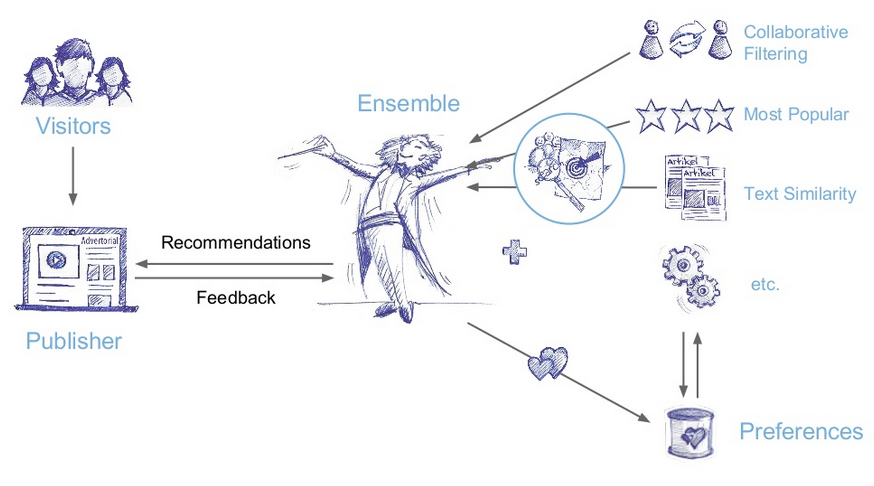
\includegraphics[width=1.0\textwidth]{obr/plistaEnsemble.png}
 	\caption[Abstraktní pohled na systém společnosti plista]{Abstraktní pohled na systém společnosti plista. Zdroj: \cite{slideshare:plista}}\label{fig:plista}
\end{figure}	

V prezentaci bylo zmíněno několik užitečných rad ohledně toho, co všechno by měl systém podobného typu umět. Zmíněna je potřeba rychlého síťového protokolu a rychlé fronty zpráv. Padla zde též potřeba rychlého úložiště pro data.

K dosažení správné funkcionality pro výběr nejlepšího algoritmu společnost používá tzv. \emph{multi-armed bayesian bandit}~\ref{sub:mabandit} v bayesovské variantě, což je i jedna ze strategií, kterou mi na úvodní schůzce doporučil vedoucí této práce.

\subsubsection{easyrec}
Technická knihovna společnosti IBM obsahuje přehledný seznam~\cite{ibm} několika doporučovacích systémů, z nichž převážná část vznikla jakou součást univerzitního výzkumu.

Z tohoto seznamu se mi jako velmi zajímavý jeví systém \textbf{easyrec}\footnote{\url{http://easyrec.org/recommendation-engine}}. Jedná se o open source webovou aplikaci napsanou v programovacím jazyce Java nabízející personalizovaná doporučení prostřednictvím RESTful webových služeb. Díky vystavenému REST API\footnote{REST API systému easyrec: \url{http://easyrec.org/implement}} je vývojáři umožněno napojit svou aplikaci psanou v libovolném jazyce na systém a využívat jejích funkcionalit. Lze tak zasílat uživatelské akce typu prohlížení, provedení nákupu či hodnocení položky a žádat o doporučení. Tyto uživatelské akce jsou ukládány do databáze easyrec.

K doporučování lze přistupovat prostřednictvím specifických endpointů, například \emph{zboží související s danou položkou}, dále \emph{ostatní uživatelé prohlíželi též tyto položky} nebo lze dostávat \emph{specifická doporučení pro daného uživatele}~\cite{ibm}. 

Systém provádí na pozadí analytické operace, obsahuje též databázi asociačních pravidel a podporu online i offline doporučování. Uživatelským aplikacím připojujícím se k systému generuje v odpovědích žádaná doporučení (viz obrázek~\ref{fig:easyrec}).

\begin{figure}\centering
	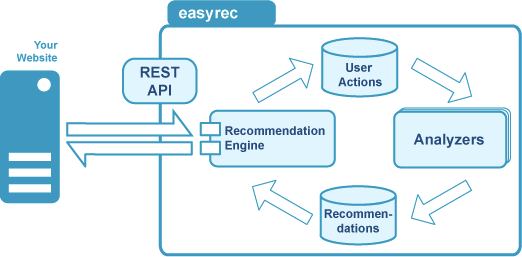
\includegraphics[width=1.0\textwidth]{obr/easyrec.png}
 	\caption[Abstraktní model open source systému easyrec]{Abstraktní model open source systému easyrec. Zdroj: \cite{easyrec}}\label{fig:easyrec}
\end{figure}	

\subsection{Shrnutí poznatků z analýzy}  

   \begin{table}
   \centering
\begin{tabular}{|c|c|}
        \hline \bfseries Systém & \bfseries Vlastnosti \\ \hline
    \hline
  \bfseries Amazon.com & 
  \begin{minipage}{3.5in}
    \vskip 6pt
    \begin{enumerate}
   \item Kolaborativní filtrování užívající podobnostní mapování item-to-item~\cite{linden2001collaborative}.
   \item Personalizovaná doporučování získávaná z databáze informací o uživatelích~\cite{jacobi2006personalized}. Informace jsou mezi sebou kombinovány za účelem vytvoření nejlepšího doporučení.
   \end{enumerate}
   \vskip 6pt
 \end{minipage}
 \\
  \hline
  
  \bfseries Netflix & 
  \begin{minipage}{3.5in}
    \vskip 6pt
    \begin{enumerate}
   \item Predikce uživatelských hodnocení založená na technikách strojového učení~\ref{sec:machine}.
   \item Pro doporučování je využíváno více jednotlivých algoritmů a jejich kombinování. Velmi záleží na tom, zda uživatel hodnotí film ráno, večer, o víkendu, kdy má volno a podobně.
   \end{enumerate}
   \vskip 6pt
 \end{minipage}
 \\
  \hline  
  
  \bfseries Mendeley & 
  \begin{minipage}{3.5in}
    \vskip 6pt
    \begin{enumerate}
   \item Doporučení založená na kolaborativním filtrování ve variantách user-based i item-based.
   \item Doporučení založená na podobnosti obsahu (podobnost článků, nadpisů, klíčových slov apod.)
   \item Důraz na pozitivní a negativní zpětnou vazbu.
   \item Výpočetní vrstva pro doporučování postavená nad Apache Mahout~\ref{mahout}. 
   \end{enumerate}
   \vskip 6pt
 \end{minipage}
 \\
  \hline    
  
  \bfseries Google News & 
  \begin{minipage}{3.5in}
    \vskip 6pt
    \begin{enumerate}
   \item Kombinování informací získaných z předchozího chování na stránce s technikami kolaborativního filtrování.
   \end{enumerate}
   \vskip 6pt
 \end{minipage}
 \\
  \hline   
  
  \bfseries ORP & 
  \begin{minipage}{3.5in}
    \vskip 6pt
    \begin{enumerate}
   \item Kombinování více doporučovacích metod společně s kontextem uživatele.
   \item Přítomnost mezivrstvy v podobě rádce starajícího se o obsluhu uživatelů a jejich doporučení.
   \item Silný důraz na zpětnou vazbu a následné přepočítávání budoucích šancí doporučení.
   \item Ke kombinaci je využíváno strategie Multi-armed bandit~\ref{sec:multi} v bayesovské variantě~\ref{bayes}.
   \end{enumerate}
   \vskip 6pt
 \end{minipage}
 \\
  \hline     
  
  \bfseries easyrec & 
  \begin{minipage}{3.5in}
    \vskip 6pt
    \begin{enumerate}
   \item Veškeré uživatelské akce (provedení akce, zpětná vazba, žádost o doporučení konkrétním algoritmem) s doporučovacím systémem probíhají skrze komunikaci s RESTful API.
   \end{enumerate}
   \vskip 6pt
 \end{minipage}
 \\
  \hline    
 \end{tabular}
     \caption {Shrnutí poznatků o jednotlivých systémech vyplývající z provedené analýzy.}
     \label{tab:table}
   \end{table} 

Z výše uvedených příkladů v sekci~\ref{sec:examples} lze vypozorovat určité vlastnosti (shrnutí v tabulce~\ref{tab:table}) a zformulovat několik závěrů:

\begin{itemize}
	\item O uživateli je vedena spousta záznamů, především historie jeho chování na stránkách.
	\item Velký důraz je kladen na zpětnou vazbu (vyjádření zájmu uživatele o doporučený obsah), ať už formou přečtení článku, ohodnocení položky apod.
	\item Stále je využíváno osvědčených metod kolaborativního filtrování a filtrování na základě obsahu.
	\item Síla není v použití jednoho konkrétního algoritmu, ale v kombinaci více metod a přístupů dohromady.
	\item Většina systémových výpočtů běží na pozadí v tom samém čase, co uživatel tráví prohlížením stránky. Systém je schopna rychle se přizpůsobit okolnostem.
	\item Problematika kombinování metod má silnou závislost na strojovém učení a teorii pravděpodobnosti a statistiky (především bayesovské).
	\item Realizace RESTful API je poměrně vhodný způsob komunikace s doporučovacím systémem ověřeným v praxi.
\end{itemize}

Existujících řešení je tedy celá řada. Každé z těchto řešení je přitom využíváno k vlastnímu účelu a není snadno přenositelné.

Potvrdila se domněnka, že době, kdy obchodníkům stačilo na svůj elektronický obchod nasadit jednoduchý algoritmus kolaborativního filtrování, odzvonilo a budoucnost patří systémům schopným predikce a přizpůsobení svého vývoje, a to vše v reálném čase. 

\section{Teorie adaptibilního systému}
\label{chap:adapt}

\subsection{Minimální teoretický základ}

Ještě předtím, než se pustím do popisu navrhované strategie, zopakuji zde některé pojmy týkající se strojového učení, teorie pravděpodobnosti a statistiky. Jedná se o minimální základ potřebný k pochopení postupů popisovaných dále v této sekci. 

\subsubsection{Strojové učení}
Strojové učení je vědecká disciplína (jedna z větví oboru umělé inteligence), jež se zabývá tím, jak se má počítač přizpůsobit určité situaci, aniž by byl pro danou situaci explicitně naprogramován. Detailněji v sekci~\ref{sec:machine}.

\subsubsection{Agent}
\label{agent}
Agent je speciální autonomní program, který jedná samostatně a nezávisle bez vedení uživatele. Jeho úkolem je komunikovat s okolím a interagovat v závislosti na okolních podnětech. Dalšími důležitými vlastnostmi jsou schopnost příhodně reagovat na danou situaci a též proaktivně vykonávat činnost a dosahovat cíle prostřednictvím vlastní iniciativy. Jedná se o definici obecnou, ale pro naše potřeby zcela dostačující.

Problematika agentů a agentních systémů je jinak samostatný obor spadající do oblasti umělé inteligence a jeho zkoumání by vydalo na další závěrečnou práci. 

\subsubsection{Zpětná vazba}
\label{feedback}
Zpětnou vazbou je označován proces, ve kterém na základě obdržených informací (například při komunikaci s nějakým systémem) a reakcí na ně ovlivňujeme jejich budoucí podobu – část systémového výstupu lze tedy použít jako vstup pro další činnost systému.

Rozlišujeme dva typy reakcí, a to kladnou zpětnou vazbu a zápornou zpětnou vazbu. Téma má blízko k psychologickému zkoumání toho, jakým způsobem dokáže ovlivnit zapojení odměny a trestu lidské chování.

\subsubsection{Explorace vs. exploatace}
\label{sub:explo}

\begin{description}
  \item[Explorace] Nacházení nových oblastí hledání, kdy agent nevyužívá předchozích znalostí (agent stále zkouší nové akce, jejichž výsledek nezná).
  \item[Exploatace] Využívání stávajících znalostí. Hrozí uváznutí v lokálních extrémech. (agent provádí akce, o kterých ví, že mu přinášejí užitek). 
\end{description}	

Optimální strategie nemůže být ani čistě explorační, ani čistě exploatační. Hledá se vyvážený kompromis.

\subsubsection{Základy teorie pravděpodobnosti}

Nejprve uvedu několik pojmů z teorie pravděpodobnosti, se kterými budu v následujícím textu pracovat.

\paragraph{Pravděpodobnostní prostor}

Pravděpodobnostní prostor prováděného náhodného pokusu je tvořen trojicí $(\Omega,\mathcal{F},P)$, kde:
	\begin{itemize}
		\item $\Omega$ je prostor elementárních jevů (např. čísla od jedné do šesti na šestistranné hrací kostce), kde elementárním jevem nazýváme libovolný možný výsledek $\omega \in \Omega$ 
		\item $\mathcal{F}$ je množina náhodných jevů (potenční množina\footnote{Potenční množina množiny $X$ je množina obsahující všechny podmnožiny množiny $X$} množiny $\Omega$)
		\item $P$ je přiřazení pravděpodobnosti jednotlivým jevům z $\Omega$ ($P(\Omega)=1$)
	\end{itemize}

\paragraph{Náhodný jev}
	
Náhodný jev $A$ výsledek náhodného pokusu. Příkladem jevu může být například hod mincí a pozorování, zda padla panna nebo orel. V tomto jevovém prostoru jsou zahrnuty celkem dva elementární jevy (hodnota panna a hodnota orel), které souvisejí s pokusem (pozorování výskytu elementárních jevů během házení).	

\paragraph{Náhodná veličina}
	\label{randomvel}
Výsledkem náhodného pokusu nemusí být číslo (v příkladu výše jsme měli dvě hodnoty po stranách mince), proto je vhodné těmto výsledkům kvůli matematickému zpracování čísla přiřazovat. Způsob přiřazení čísla výsledku náhodného pokusu se označuje jako \emph{náhodná veličina $X$}~\cite{pst1}. Pro počítání padlých panen při opakovaném házení mincí by mohlo přiřazení vypadat například takto:

\begin{itemize}
	\item $X(panna) = 1$
	\item $X(orel) = 0$
\end{itemize}

Náhodná veličina na pravděpodobnostním prostoru $(\Omega,\mathcal{F},P)$ je tedy funkce $X: \Omega \to R$, která každému $\omega \in \Omega$ přiřadí $X(\omega)$ a pro kterou platí podmínka měřitelnosti:

\begin{center}
$\{ X \leq x \} = \{ \omega \in \Omega: X(\omega) \leq x \} \in \mathcal{F}, \forall x \in R$
\end{center}

Dle typu se rozlišují náhodné veličiny diskrétní a spojité. Diskrétní náhodné veličiny mohou nabývat pouze konečného počtu hodnot z $R$ (například ročník studia), zatímco spojité náhodné veličiny nabývají v určitém intervalu libovolné reálné hodnoty (například čas potřebný k dokončení diplomové práce). 

Pravděpodobnostní rozdělení náhodné veličiny určuje její distribuční funkce. 

\subsubsection{Distribuční funkce}
\label{cdf}
Distribuční funkce náhodné veličiny $X$ je funkce $F: R \to \langle0,1\rangle$ definovaná vztahem 

\begin{center}
$F(x) = P(X \leq x) = P(\{ \omega \in \Omega: X(\omega) \leq x \})$.
\end{center}

Vyjadřuje tedy pravděpodobnost, že hodnota náhodné veličiny $X$ nabude hodnoty menší nebo rovné zadané hodnotě (libovolnému $x \in R$). Distribuční funkce určuje rozdělení pravděpodobnosti.

\subsubsection{Kvantilová funkce}
\label{icdf}
\cite{pst2} Podobně jako distribuční funkce, i kvantilová funkce se týká rozdělení pravděpodobnosti. Lze ji považovat za funkci inverzní k distribuční funkci, neboť zatímco distribuční funkce $y = F(x)$ vyjadřuje pravděpodobnost, s jakou bude hodnota náhodné veličiny $X$ menší nebo rovna $x \in R$, výsledkem kvantilové funkce $x = F(y)^{-1}$ je hodnota $x$, pro jakou je výsledek náhodného pokusu se zadanou pravděpodobností $y$ menší nebo roven $x$. Jinými slovy hledáme taková $x$, kterým odpovídá určitá hodnota distribuční funkce $F(x)$. Hodnoty této funkce jsou tedy \emph{kvantily}.

\subsubsection{Rozdělení pravděpodobnosti}
\label{distr}
Někdy se též označuje jako distribuce pravděpodobnosti náhodné veličiny $X$. 
Rozdělení pravděpodobnosti každému jevu popsanému veličinou $X$ přiřazuje určitou pravděpodobnost. V diskrétním případě přiřazujeme pravděpodobnosti jednotlivým hodnotám (lze si představit jako samostatné body v grafu), ve spojitém případě pak intervalu hodnot náhodné veličiny. 

Rozdělení pravděpodobnosti je celá řada, z diskrétních je známé například \emph{binomické} ($n$ pokusů s rovnocennou pravděpodobností) či \emph{geometrické} rozdělení. Ze spojitých například \emph{normální rozdělení}, \emph{exponenciální rozdělení} nebo \emph{beta rozdělení}.

\subsubsection{Beta rozdělení}
\label{beta}
Beta rozdělení ${Beta}(\alpha, \beta)$ je spojité pravděpodobnostní rozdělení definované na intervalu $\langle0,1\rangle$. Rozdělení má dva vstupní parametry $\alpha$ a $\beta$ určující tvar. Rozdělení se používá k modelování chování náhodných veličin, které jsou omezené na konečné intervaly. 

\subsubsection{Bayesovská statistika}
Jedná se o moderní větev statistiky pracující s podmíněnou pravděpodobností. Základem bayesovské statistiky je známý \emph{Bayesův teorém} (často označovaný jako Bayesova věta) vyjadřující pravděpodobnost hypotézy ($H_j$) v závislosti na datech ($D$) a případně modelu ($M$). Lze pomocí ni stanovit pravděpodobnost, aniž bychom měli k dispozici známá fakta z minulosti. Oproti klasické statistice taktéž netestujeme hypotézy, ale provádíme \emph{odhady}. 

\subsubsection{Apriorní pravděpodobnost (prior)}
\label{prior}
Pravděpodobnost $P(H_j | M)$, označována jako \emph{prior}. Značí to, co víme nebo si myslíme předem, ještě před získáním dat (např. výsledky předchozích experimentů)~\cite{pst4}. Lze jí vyjádřit určitou míru nejistoty, například podíl voličů, kteří budou v budoucích volbách hlasovat pro nějakého konkrétního politika. 

\subsubsection{Aposteriorní pravděpodobnost (posterior)}
\label{poster}
Pravděpodobnost $P(H_j | D, M)$, označována jako \emph{posterior}. Udává výsledek celého snažení, tedy pravděpodobnost naší hypotézy v závislosti na předchozích znalostech (prior) a současně nových datech~\cite{pst4}.

Díky uvedeným pravidlům je možné s každou další objevenou skutečností zpřesňovat pravděpodobnost výchozí hypotézy. 

\subsubsection{Náhodný výběr}
\label{randomvyber}
Náhodného výběru se využívá k rozpoznání charakteru rozdělení (opakované pokusy dávají za stejných podmínek různé výsledky, které odpovídají hodnotám jednotlivých realizací náhodné veličiny). Jedná se o uspořádanou $n$-tici ($X_1$, $X_2$, \ldots, $X_n$) náhodných veličin $X_i$, $1 \leq i \leq n$, které jsou nezávislé a mají stejné rozdělení pravděpodobnosti~\cite{pst3}.

Zatímco \textbf{náhodným výběrem} označujeme $n$-prvkovou posloupnost nezávislých náhodných veličin $X_1$, $X_2$, \ldots, $X_n$, pojmem \textbf{výběr} budeme značit $n$-prvkovou posloupnost reálných čísel $x_1$, $x_2$, \ldots, $x_n$~\cite{pst5}. 

\subsubsection{Statistická inference}
\label{inferno}
\cite{pst5} Uvažujme pojem \emph{populace}, kdy populací myslíme náhodnou veličinu s jejím rozdělením pravděpodobnosti. Úkolem statistické inference je pak s použitím \textbf{výběru} z populace \emph{odhadnout parametr}, neboli číselnou hodnota platící pro celou populaci (tou může být například střední hodnota rozdělení, rozptyl a tak podobně).

Odhadem je myšleno získání číselné hodnoty nebo intervalu hodnot z výběru. Cílem je, aby měl takový odhad blízko skutečné hodnotě parametru.

Rozlišujeme dva typy odhadů, a to bodový, kdy odhadem je jedna hodnota, a intervalový, kdy je odhadem interval hodnot. 

\subsubsection{Multi-armed Bandits}
\label{sub:mabandit}
Jeden z klasických učících problémů zasahující do teorie pravděpodobnosti. Herní strategie je podobná filosofii tradičního výherního automatu (představujícího \emph{one-armed strategii}) s tím rozdílem, že multi-armed varianta má více herních pák, a proto lze v každém kole pro jednu hru volit mezi více automaty. Strategií se detailněji zabývá sekce~\ref{sec:multi}.

S pojmy vysvětlenými výše souvisí strategie v tom smyslu, že použitím bayesovské varianty provádíme opakovaný výběr z konečného počtu rozdělení, čímž se snažíme maximalizovat průměrnou hodnotu.

Toho lze využít například k cílenému doporučování reklamy nebo výběru personalizované úvodní stránky pro uživatele vstupujícího na naše stránky. Což je vlastně analogie k problému řešeného v této práci.

\subsection{Význam strojového učení}
\label{sec:machine}

Jak vyplynulo z rešerše~\ref{chap:current} existujících řešení, vzhledem k povaze řešeného problému je nutné zaměřit se na metody \emph{strojového učení}. 

Těmito metodami lze dosáhnout generalizace vstupních instancí na správné výsledky nebo adaptovat existující systém na změny a reakce okolí. 

Typickým příkladem je vytvořit z dostupných dat model, jenž například dokáže:

\begin{itemize}
  \item predikovat cenu akcií za 6 měsíců (z aktuální výkonnosti společnosti a dostupných ekonomických dat),
  \item rozpoznat spam od regulérního e-mailu,
  \item u pacienta hospitalizovaného s infarktem predikovat riziko dalšího infarktu,
  \item napomoci společnostem zabývajících se internetovou reklamou v rozhodování se, kterou reklamní strategii použít k maximalizaci zisku.
\end{itemize}

Algoritmy strojového učení dělíme do taxonomie (nadtříd a podtříd) založené na požadovaném výsledku nebo typu vstupu, jenž máme k dispozici během trénování stroje. Algoritmů je celá řada, zmíním zde alespoň ty nejtypičtější. 

\begin{description}
  \item[Supervised learning]\footnote{učení s učitelem} je typ učení, které se používá v případě, že máme k našim trénovacím instancím na vstupu korektní výsledky. Pomocí kombinace trénovacích vstupních instancí a jejich požadovaných výsledků lze systém adaptovat na situaci, že dokáže sám předpovídat výsledky pro každé další platné vstupní instance~\cite{aihorizon}.
  
  Využití nachází například v oblastech rozpoznávání řeči či detekci spamu.
  \item[Unsupervised learning]\footnote{učení bez učitele} je již ze samotné podstaty absence učitele obtížným problémem. Učení bez učitele se používá k analýzu dat, když nemáme k dispozici informace od učitele (trénovací množinu). Pozorovaná data se mají vysvětlit pomocí matematických modelů.
  
  Používá se v oblasti rozpoznávání vzorů~\cite{hlavac}.
  \item[Reinforcement learning]\footnote{zpětnovazební učení nebo též učení posilováním} je oblast informatiky tykající se chování agentů~\ref{agent}. Jedná se o metodu, při které se agent učí, jakým způsobem má volit akce, aby nalezl optimální strategii pro dané prostředí.
  
  Jedná se o učení bez učitele. Agent sice dostává odezvu, ale přímo z prostředí, takže musí experimentovat a zjišťovat, které stavy jsou nějakým způsobem dobré, a kterým stavům je lepší se vyhnout.
  
  Průzkum probíhá na principu zpětné vazby~\ref{feedback} v podobě odměny za akce dosahující cíle nebo trestu v opačném případě. Řeší se zde problém explorace vs. exploatace~\ref{sub:explo}. 
\end{description}

Rozlišujeme několik typů zpětnovazebního učení, například tzv. \emph{single-stage} (agent se snaží uplatňovat zpětnou vazbu ihned po každé provedené akci), oproti kterému stojí typ \emph{sekvenční} (agent uplatňuje zpětnou vazbu po obdržení série akcí). Dalšími typy jsou pak například \emph{pasivní} a \emph{aktivní} zpětnovazební učení přizpůsobující svůj vývoj na základě pevně dané strategie, respektive učení se a rozhodování o prováděných akcích za chodu systému~\cite{reinforcement}.

Algoritmus zpětnovazebního učení začíná při svém spuštění ve stavu nevědomí, kdy neví nic o daných okolnostech a začíná nabývat své vědomosti postupným testováním systému. Postupující dobou běhu (a tím, jak vstřebává data a vyhodnocuje výsledky) se učí rozpoznat, jaké chování je nejlepší.

\subsubsection{Zvolená strategie učení}
\label{sub:online}
Za nejvhodnější strategii, která by byla schopna plnit požadavky definované na tuto práci, jsem zvolil \emph{algoritmus zpětnovazebního učení}.

O strategii lze též mluvit jako o \emph{online učení}. Nutno zmínit, že slovem online zde není míněno něco ve smyslu internetu, ale ve smyslu neustále se vyvíjející aktualizace dat. Učící algoritmus v každém kole vykoná nějakou akci, přijme zpětnou vazbu a připíše si daný zisk či ztrátu.

Z matematického hlediska má online učení propojení na klasické online algoritmy, teorii (opakovaných) her a teorii pravděpodobnosti.

Díky těmto znalostem tak můžeme navrhovat pravděpodobností dynamické systémy, kterými lze modelovat složitá průmyslová zařízení nebo třeba výherní automat známý jako \emph{Multi-Armed Bandit}.

\subsection{Multi-armed Bandits algoritmus}
\label{sec:multi}

\subsubsection{Princip algoritmu}
Základ algoritmu si lze představit tak, že hráč stojí před $N$ výherními automaty (ty jsou podle dle strategie nazývány jako bandité) a v každém kole má možnost vybrat si jeden, na kterém bude hrát.

Strategie je formálně popsána jako skupina výnosových distribučních funkcí~\ref{cdf} $B = \{ A_1, A_2, \ldots, A_N \}$, kde $N$ je počet banditů (každý z banditů má tedy přiřazenu právě jednu distribuční funkci vyjadřující pravděpodobnost úspěchu). 

Hráč zpočátku nedisponuje žádnou informací o průběhu hry, ani o rozložení pravděpodobnosti úspěchu mezi bandity, a maximalizace výhry může dosáhnout pouze tím, že v každém kole vhodně vybere vždy jednoho z banditů.

Kdyby hráč věděl, u kterého z banditů je největší pravděpodobnost výhry, samozřejmě by vždy vybíral právě tohoto. Pravděpodobnosti výher u jednotlivých automatů jsou ale neznámé.

\paragraph{Přizpůsobení algoritmu pro potřeby adaptibilního systému}
Tradiční varianta pracuje s předem definovaným počtem tahů, kterými je celá hra omezena. Úkolem hráče tedy je nalézt nejlepšího banditu, a to tak rychle, jak jen to je možné, aby jej stihl využít co nejvíce~\cite{camdp}.

Vzhledem k povaze mnou řešeného problému, kdy je cílem navrhnout a vyvinou rádce, jenž naslouchá a odpovídá pouze tedy, kdy je vyzván uživatelem, je chování systému zhruba takové:

\begin{itemize}
	\item Rádce může udělovat rady klidně až do nekonečna. Pokud ale nebude dostávat pravidelnou zpětnou vazbu o výsledcích svých rad, budou jeho rady čistě náhodné.
	\item Zpětnou vazbu mu poskytují uživatelé, kteří u něj žádají o radu. Uživatelé poskytují informace dvojího typu – zda se \emph{řídili při volbě algoritmu jeho radou} a zda byli \emph{po doporučení obsahu s výsledkem spokojeni či nikoliv}.  
\end{itemize}

Popisu toho, jaký vliv má zpětná vazba na vývoj samotného systému, se věnuje příslušná podpodkapitola~\ref{subsub:feedback}.

\paragraph{Návrh strategie učení}
	
Návrh strategie spočívá v tom, že systém (rádce) jednotlivé bandity nejdříve testuje~\ref{inferno} za účelem získání znalostí nutných pro další vývoj. Jakmile nabude více znalostí, je možné zaměřit se na bandity, kteří poskytují díky zužitkovaným znalostem největší odměnu. 

Úkol je komplikován stochastickou povahou banditů. Suboptimální bandita může přinášet spoustu výher, což by nás mohlo přimět uvěřit, že právě tento bandita je tím nejlepším. Podobně ale uvažovat i naopak – nejlepší bandita totiž může zpočátku přinášet spoustu proher.

Na místě jsou dvě otázky:

\begin{itemize}
	\item Měli bychom dávat stále šanci i banditům, u kterých často prohráváme, nebo na ně zanevřít a štěstí zkoušet u jiných?
	\item Pokud nalezneme banditu, který nám přináší \emph{docela dobré} výsledky, měli bychom se s ním spokojit a nadále maximalizovat svou výhru pouze u něj? Nebo se vyplatí zkoušet i nadále další bandity v naději, že se povede nalézt ještě lepšího?
\end{itemize}

Tato dilemata jsou odborně nazývána jako \emph{explorace a exploatace}~\ref{sub:explo}.	

\subsection{Bayesian Bandits}
\label{bayes}
Nalézt optimální řešení tedy nepatří k triviálním problémům. Systému může trvat léta, než se k němu dopracuje. Naštěstí existuje spousta \emph{přibližně optimálních} řešení.

Jedním z řešení je algoritmus zvaný \emph{Bayesian Bandits}. Algoritmus přímo souvisí s učením založeným na zpětné vazbě~\ref{feedback}.

Bayesovské řešení začíná prior~\ref{prior} stanovením pravděpodobností výhry pro každého banditu. Hodnoty jsou v rozmezí $\langle0,1\rangle$. Jak již bylo řečeno, každého banditu reprezentuje jedna distribuční funkce.

V každém kole, kterých je v případě mnou vytvářeného systému nekonečně (neboť kola jsou závislá na žádostech uživatelů, kteří přistupují k systému – standardní použití Multi-armed Bandits pracuje s konečným počtem stavů), probíhá následující proces:

\begin{enumerate}
	\item pro každého z $N$ banditů proveď prior~\ref{prior} (počty pokusů, výher, \ldots) výběr z náhodné veličiny $X_b$~\ref{randomvel} bandity $b$
	\item ze získaných dat vyber~\ref{randomvyber} banditu s největší hodnotou předchozího výběru, například $B = argmax X_b$	
	\item pozoruj výsledek vrácený banditou $B$ a proveď prior aktualizaci tohoto bandity.
	\item vrať se na krok 1
\end{enumerate}

Počáteční prior pravděpodobnost je u každého bandity Beta rozdělení~\ref{beta} ${Beta}(\alpha = 1, \beta = 1)$ (uniformní rozdělení).

Pozorovaná náhodná veličina $X$ (výhra či prohra, tedy 1 nebo 0) je binomická. Posterior~\ref{poster} pravděpodobnost se po provedení pokusu přizpůsobuje novému rozdělení:

\begin{center}
${Beta}(\alpha = 1 + X, \beta = 1 + 1 - X)$.
\end{center}

V případě jakéhokoliv úspěchu se provádí navýšení pravděpodobnosti, se kterou bude algoritmus znovu vybrán. V případě neúspěchu se tato pravděpodobnost exponenciálně snižuje. V každé další hře se již systém rozhoduje s touto pravděpodobností (mezí explorací a exploatací).

Pokud tedy chceme odpovědět na dřívější otázku, zda bychom měli dávat stále šanci i banditům, u kterých často prohráváme, nebo na ně zanevřít a zkoušet štěstí u jiných, tento algoritmus nám navrhuje to, abychom prohrávající bandity přímo nevyřazovali, ale vybírali je stále méně častěji, jakmile získáme dostatek jistoty, že existují i lepší bandité. 

Existuje tu nenulová šance, že prohrávající bandita dosáhne statusu $B$, pravděpodobnost této šance se ale snižuje s rostoucím počtem odehraných kol. 

Obrázek~\ref{fig:posteriors} znázorňuje postup pro problém tří banditů ($N = 3$), jakým se algoritmus učí s rostoucím počtem her. Přerušované čáry pod grafy hustoty každého rozdělení reprezentují skryté reálné pravděpodobnosti (v obrázku mají hodnoty $0.85$, $0.60$, $0.75$). Z uvedeného příkladu vyplývá, že o skryté pravděpodobnosti se až tolik nestaráme. Daleko větší význam pro nás má výběr nejlepšího bandity, což je vidět na distribuci červeného bandity. Ta je velice široká, což představuje skutečnou neznalost o tom, jak velkou skrytou pravděpodobností bandita disponuje. O pravděpodobnosti tedy nemáme nejmenší tušení, jsme si ale docela jistí tím, že bandita není nejlepší. Algoritmus se proto rozhodne ignorovat jej.

\begin{figure}\centering
	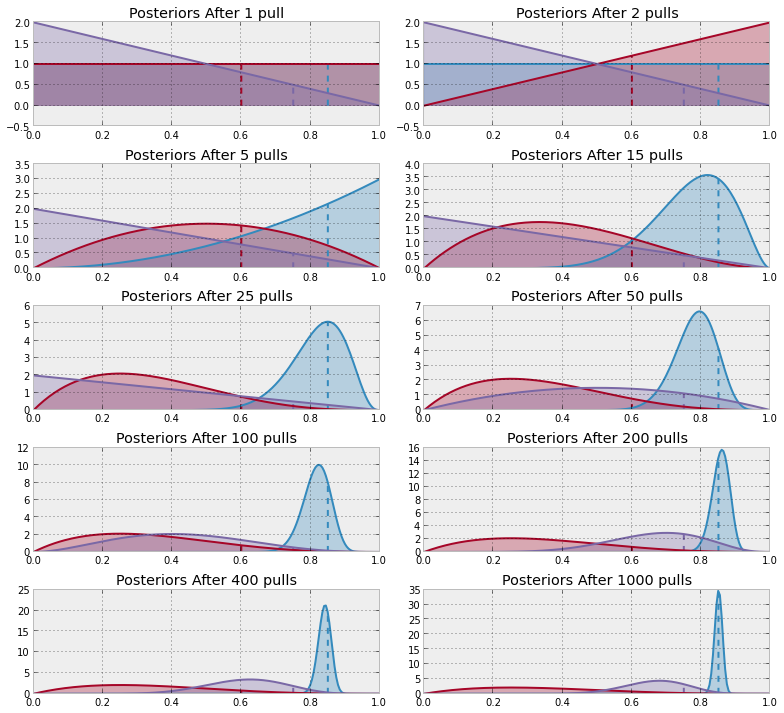
\includegraphics[width=1.0\textwidth]{obr/posteriors.png}
 	\caption[Vizualizace sekvenčního učení řešení od jedné do tisíce her.]{Vizualizace sekvenčního učení řešení od jedné do tisíce her. Zdroj: \cite{camdp}}\label{fig:posteriors}
\end{figure}	

\subsubsection{Zpětná vazba a její vliv na vývoj adaptibilního systému}
\label{subsub:feedback}
Pojem zpětné vazby~\ref{feedback} již v předchozím textu zazněl. Pro účely této práce je nutné uzpůsobit její význam tak, aby měla přímý vliv na pružný vývoj adaptibilního systému.

Vzhledem k tomu, že rádce bude plnit svůj úkol pomocí algoritmu Bayesian Bandits využívající ${Beta}$ rozdělení pravděpodobnosti (navíc operuje s pravděpodobnostmi \emph{prior} a \emph{posterior}), zpětná vazba bude mít vliv na oba parametry vstupující do rozdělení, což má ve finále vliv na tvar celé distribuce~\ref{distr} (k vidění na obrázku~\ref{fig:posteriors}). 

Jak již bylo řečeno, zpětná vazba je dvojího typu:

\begin{itemize}
	\item Informace o zvolení rádcem navrženého algoritmu pro vlastní doporučení (rádci sdělujeme, že jsme se \textbf{pokusili} řídit jeho radou).
	\item Zpětná vazba týkající se spokojenosti doporučení (zda byl tento algoritmus při doporučení \textbf{úspěšný} či nikoliv).
\end{itemize}

Do ${Beta}$ rozdělení vstupují dva parametry – $\alpha$ a $\beta$.

Při každé žádosti na rádce je tedy pro každého banditu $B_i$ provedeno posterior (značením $B_i(success)$ se snažím naznačit dosavadní míru úspěchů bandity $B_i$, pomocí $B_i(trials)$ zase dosavadní míru pokusů téhož bandity):

\begin{center}
${Beta}(\alpha = 1 + B_i(success), \beta = 1 + B_i(trials) - B_i(success))$.
\end{center}

Na ukázku jsem připravil dva příklady posterior hustoty rozdělení pravděpodobnosti dle různých vstupních parametrů vstupujících do rozdělení ${Beta}$. Obrázek~\ref{fig:beta1} znázorňuje situaci 4 úspěchů ze 4 pokusů, zatímco obrázek~\ref{fig:beta2} 1 úspěch ze 4 pokusů. Na druhém obrázku lze vidět, že distribuce je širší.

\paragraph{Typy zpětné vazby pro adaptibilní systém}

\begin{itemize}
	\item Informace o zvolení algoritmu přičte k míře pokusů tohoto algoritmu (bandity) hodnotu. Ostatním algoritmům se nic přičítat ani odečítat nebude.
	\item V případě pozitivní zpětné vazby bude zvolenému algoritmu přičtena hodnota k míře jeho úspěchu. Ostatním algoritmům bude od této míry v poměru odečteno nebo bude poměr zachován.
	\item V případě negativní zpětné vazby bude zvolenému algoritmu odečtena hodnota z míry jeho úspěchu. Ostatním algoritmům bude hodnota přičtena nebo nezměněna.
\end{itemize}

\textbf{Stanovení nejvhodnějších hodnot a konkrétního přístupu bude provedeno na základě experimentů.}

\begin{figure}\centering
	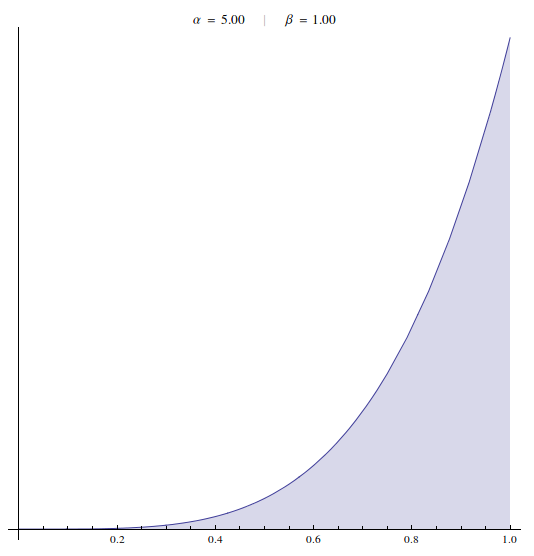
\includegraphics[width=1.0\textwidth]{obr/beta1.png}
 	\caption[Hustota pravděpodobnosti $Beta$ rozdělení pro vizualizaci 4 úspěchů ze 4 pokusů.]{Hustota pravděpodobnosti $Beta$ rozdělení pro vizualizaci 4 úspěchů ze 4 pokusů.}\label{fig:beta1}
\end{figure}	

\begin{figure}\centering
	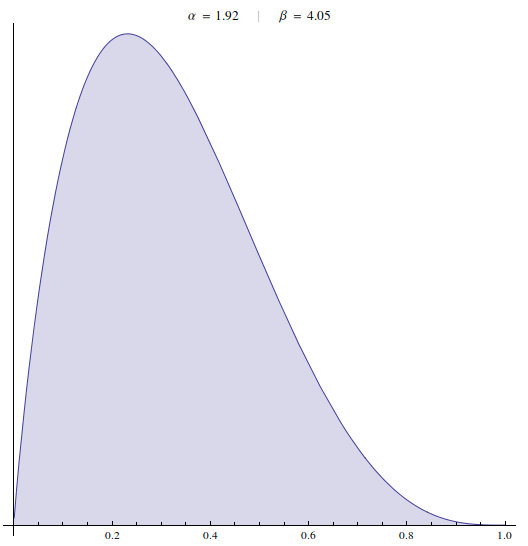
\includegraphics[width=1.0\textwidth]{obr/beta2.png}
 	\caption[Hustota pravděpodobnosti $Beta$ rozdělení pro vizualizaci 1 úspěchu ze 4 pokusů.]{Hustota pravděpodobnosti $Beta$ rozdělení pro vizualizaci 1 úspěchu ze 4 pokusů.}\label{fig:beta2}
\end{figure}	

\subsubsection{Stanovení míry učení}
\label{rate}
Vzhledem k tomu, že prostředí se mění velmi rychle v čase, je nutné stanovit nějakou míru učení, Technicky vzato je standardní Bayesian Bandits algoritmus schopen vyvíjet se sám díky neustálé aktualizaci parametrů vstupujících po každé provedené akci do ${Beta}$ rozdělení.

Stanovením vhodné míry učení lze ale docílit toho, že algoritmus se bude přizpůsobovat měnícímu se prostředí rychleji a bude fungovat též jako prevence proti vyčerpání hodnot datových typů programu.

Pokud stanovíme míru $<$ 1, algoritmus bude předchozí výsledky zapomínat rychleji a častěji bude zkoumat nové možnosti. Míra $>$ 1 implikuje naopak to, že algoritmus bude sázet na časnější dřívější výhry, čímž ale riskuje to, že se nedokáže rychle adaptovat na náhlé změny (je více imunní vůči rychle se měnícímu prostředí).

Míra $<$ 1 bude pro potřeby adaptibilního systému vhodnější. Konkrétní hodnotu se opět pokusím stanovit v závislosti na provedených experimentech.

\subsection{Význam pro kombinování}
\label{lkombinování}
Význam bayesovské strategie pro kombinování spočívá ve výběru správné metody, která bude přidána do množiny ostatních vybraných metod. Z této množiny metod je dále nutné vybrat nejvhodnější a tu použít.

Jako nejefektivnější a zároveň nejjednodušší postup se jeví výběr metody s největší četností výskytu. 

V případě shody, kdy bude mít více metod stejnou četnost výskytu, bude učiněna volba jedné konkrétní pseudonáhodně.

\chapter{Praktická část}
\label{chap:prakt}
\section{Analýza a návrh řešení}
\label{chap:analysis}
Náplní této sekce je sepsání požadavků na systém, které vyplynuly z úvodních konzultací s vedoucím práce a též vlastním zkoumáním řešeného problému. Se znalostí těchto požadavků pak bude možné provést hrubý návrh architektury systému včetně technického řešení komponent, kterými bude systém disponovat.

S ohledem na výstupy získané v této kapitole by mělo být možné provést implementaci systému.

\subsection{Požadavky}
\label{sec:req}
Za účelem vyšší přehlednosti jsem se rozhodl související požadavky strukturovat do zastřešujících skupin dle části aplikace, která bude mít jejich obsluhu na starosti.

Vyvíjenými částmi jsou:

\begin{itemize}
  \item \textbf{Adaptibilní systém pro doporučování obsahu,}
  \item \textbf{Sada základních algoritmů určených k doporučování,}
  \item \textbf{RESTful API pro manipulaci s doporučovacími algoritmy a systémem.}
  \item \textbf{Klientská aplikace pro simulaci modelové úlohy.}    
\end{itemize}

\subsubsection{Požadavky na adaptibilní systém}

\begin{itemize}
	\item Systém poklade důraz na zpětnou vazbu, pomocí které bude přizpůsobovat své chování.
	\item Systém bude přijímat zpětnou vazbu v podobě informace o tom, že uživatel se rozhodl využít jeho rad.
	\item Systém bude přijímat pozitivní (v případě dobrého doporučení) a negativní (v případě nevhodného doporučení) zpětnou vazbu.
	\item Systém bude v pravidelných intervalech ukládat do databáze svůj aktuální vnitřní stav.
	\item Systém bude schopen v případě pádu aplikace a po jejím opětovném spuštění načíst naposledy uložený vnitřní stav.
	\item Systém bude veškeré své operace týkající se rad a doporučování provádět a vyhodnocovat v reálném čase.
	\item Systém bude schopen automaticky se přizpůsobovat vývoji v čase normalizováním ukládaných hodnoty.
	\item Systém bude na každou klientskou žádost vracet příslušnou odpověď (i chybovou) – neexistuje nic jako odpověď \emph{null}.	
	\item Systém bude umožňovat vytváření a uchovávání kontextových kolekcí určených pro kombinování.
	\item Systém bude umožňovat vytváření a uchovávání kolekcí složených z existujících kontextových kolekcí určených pro kombinování.	
	\item Systém bude schopen odpovídat na žádosti uživatelů poptávajících způsob doporučení.
	\item Systém bude schopen odpovídat na další dotazy týkající se kolekcí (jejich existence apod.).	
	\item Systém bude umožňovat asynchronní komunikaci s klienty.
\end{itemize}

\subsubsection{Požadavky na sadu základních algoritmů}
\begin{itemize}
	\item Algoritmus bude dle typu přijímat parametry (uživatel, limit navrácených položek atd.), a ty využívat pro svá doporučení.
	\item Algoritmus bude komunikovat s daty uložených v Apache Solr a nad těmito daty provádět doporučovací operace.
\end{itemize}

\subsubsection{Požadavky na RESTful API}
\begin{itemize}
	\item Skrze rozhraní bude možné vytvářet kontextové kolekce se seznamem algoritmů určených pro kombinování a následnou predikci.
	\item Skrze rozhraní bude možné vytvářet kolekce složené z existujících kontextových kolekcí určených pro kombinování a následnou predikci.
	\item Skrze rozhraní bude možné vypsat existující kolekce v systému.		
	\item Skrze rozhraní bude možné zaslat systému žádost o radu a obdržet informaci o nejvhodnější metodě pro doporučení.
	\item Skrze rozhraní bude možné zaslat systému informaci o zvolené metodě pro doporučení.
	\item Skrze rozhraní bude možné zaslat systému žádost o doporučení zvolenou metodou.	
	\item Skrze rozhraní bude možné zaslat systému zpětnou vazbu týkající se spokojenosti s metodou, kterou jim byl doporučen obsah.
	\item Skrze rozhraní bude možné zaslat systému zpětnou vazbu týkající se hodnocení doporučených položek (informace, že jeden konkrétní uživatel dělá něco s jedním konkrétním dokumentem).
	\item Skrze rozhraní bude možné vytvářet v úložišti dat položky určené k doporučování. 
	\item Skrze rozhraní bude možné mazat v úložišti dat položky již nerelevantní pro doporučování. 
\end{itemize}

\subsubsection{Klientská aplikace}
\begin{itemize}
	\item Klientská aplikace se bude připojovat k výše uvedeným funkcím systému a zpracovávat získané výsledky.
	\item Klientská aplikace bude umožňovat přístup více uživatelů k systému.	
\end{itemize}	

Dle disciplín softwarového inženýrství lze výčet uvedený výše označit za \textbf{funkční požadavky}.

Definujme nyní i tzv. \textbf{nefunkční požadavky}, které specifikují vlastnosti a omezující podmínky kladené na systém:

\begin{itemize}
	\item Systém bude postaven na platformě Java.
	\item Pro uchování informací o uživatelích, položkách a jejich vzájemné interakci bude využita platforma pro vyhledávání v textu Apache Solr.
	\item Systém bude umožňovat přístup aplikacím třetích stran prostřednictvím RESTful webových služeb.
	\item Systém bude postaven tak, aby se dal snadno parametrizovat. 
	\item Systém bude připraven na situaci, že jej bude využívat více uživatelů současně.
	\item Systém poběží jako samostatná aplikace na serveru naslouchající na TCP portu. Veškerá komunikace s ní bude probíhat formou zasílání zpráv a volání procedur.
	\item Pro snadné nasazení a testování systému na libovolné pracovní stanici bude nutné vytvořit Chef cookbook/recipe\footnote{\url{http://community.opscode.com/}}.
\end{itemize}

\subsection{Architektura doporučovací platformy}

Pro zdárnou implementaci platformy splňující všechny požadavky vzešlé z analýzy výše je třeba důkladně zvážit, jaké komponenty bude obsahovat.

Diagram~\ref{fig:recommeng} znázorňuje abstraktní návrh architektury takové platformy. Mou snahou bylo zachytit přítomnost jednotlivých komponent v systému, formu jejich vzájemné komunikace a spolupráce a též základní interakci uživatele se systémem.

\begin{figure}\centering
	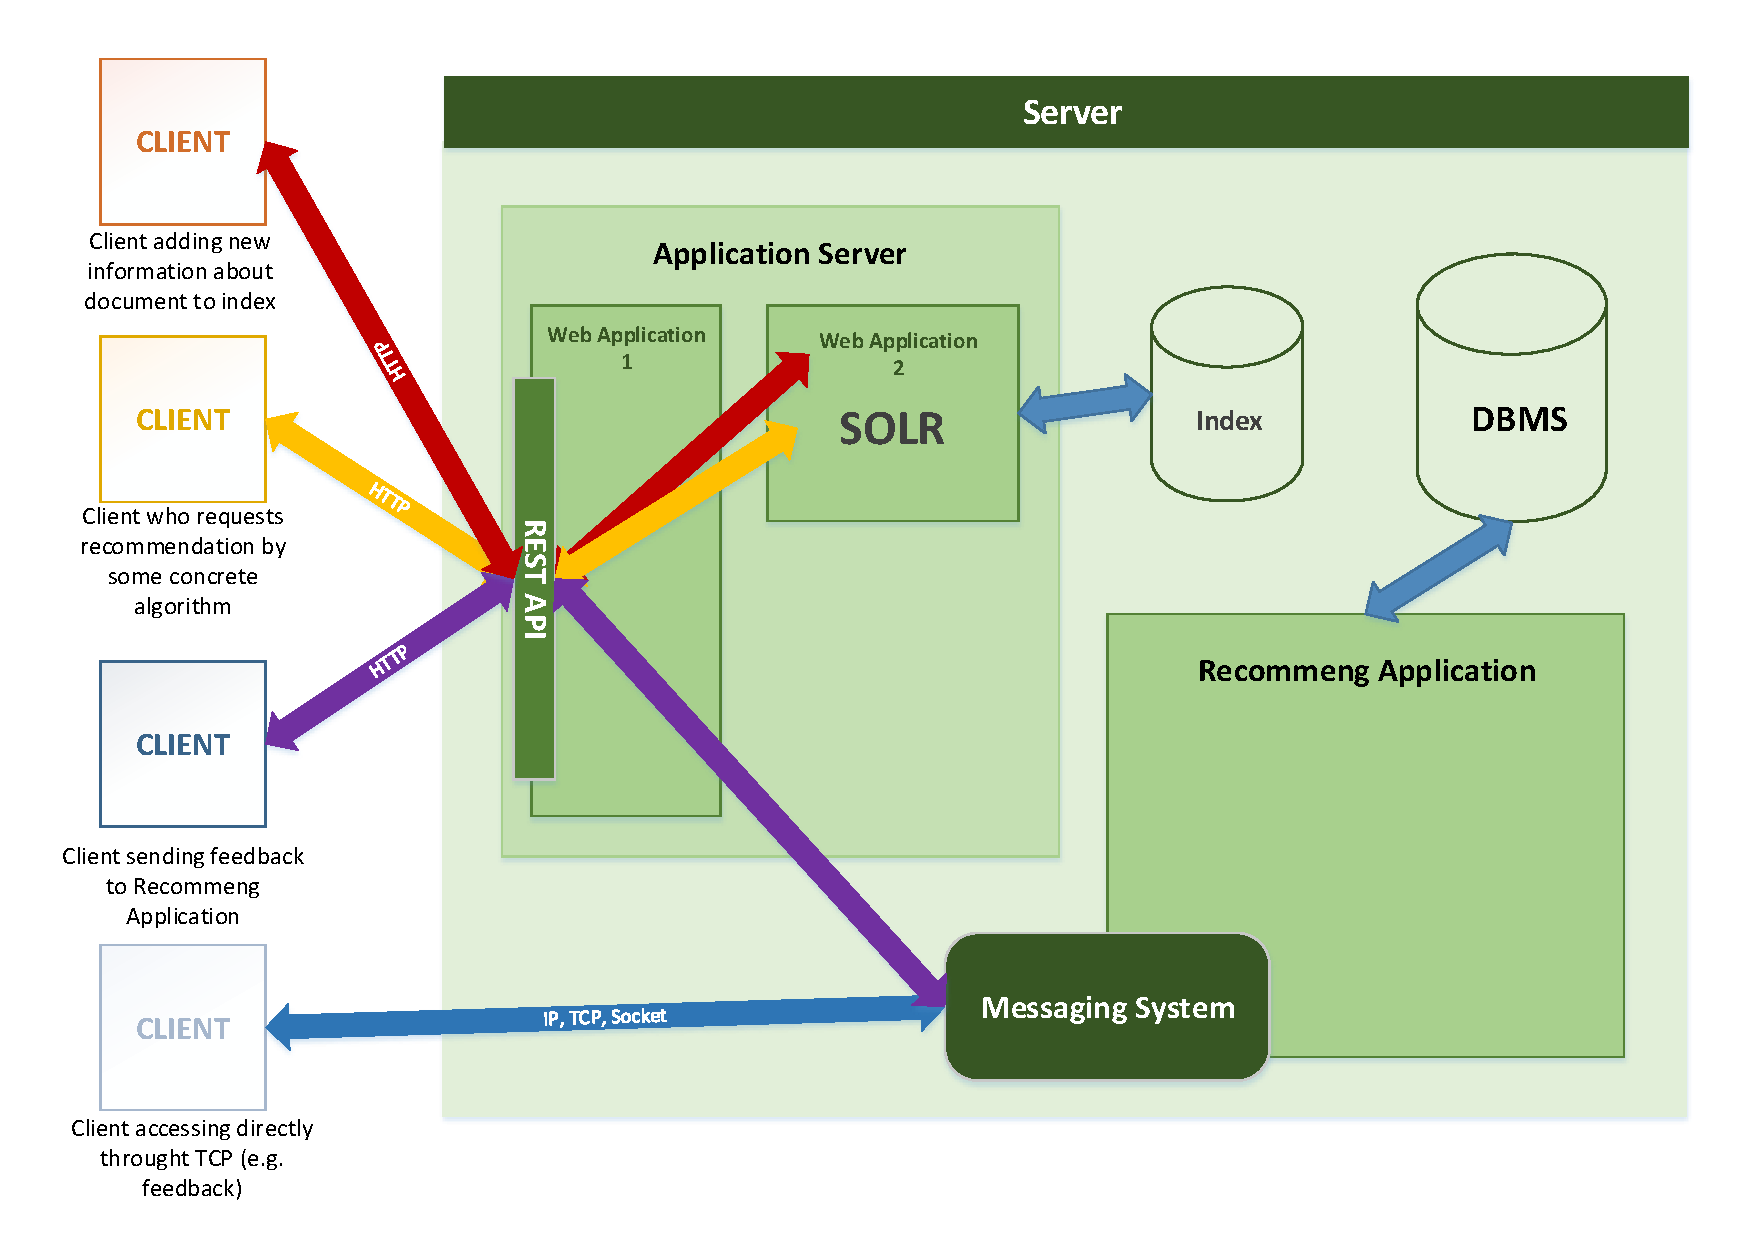
\includegraphics[width=1.0\textwidth]{obr/DIPLOMKA_env.pdf}
 	\caption[Abstraktní návrh architektury a komponent adaptibilního systému]{Abstraktní návrh architektury a komponent adaptibilního systému, ve kterém je též vidět základní interakce uživatele se systémem.}\label{fig:recommeng}
\end{figure}	

\subsubsection{Server}
Navrhovanými komponentami pro spuštění a běh na serveru jsou:

\paragraph{Webová aplikace s rozhraním pro komunikaci s klienty.}
	Viz diagram~\ref{fig:recommeng}, komponenta \emph{Web Application 1}. Aplikace bude mít na starosti obsluhu klientských požadavků na systém prováděných prostřednictvím protokolu HTTP. Zároveň bude disponovat sadou algoritmů, které lze použít pro doporučení obsahu. Dále bude aplikace obstarávat komunikační režii s druhou aplikací běžící na aplikačním serveru (\emph{Web Application 2}), kterou je platforma pro vyhledávání v textu – Apache Solr.

\paragraph{Apache Solr}
	Viz diagram~\ref{fig:recommeng}, komponenta \emph{Web Application 2}. Přítomnost této aplikace vychází z nefunkčních požadavků. Apache Solr funguje jako samostatná komponenta umožňující fulltextové vyhledávání (detaily v kapitole~\ref{chap:impl}).

\paragraph{Databáze}

Kvůli potřebě ukládat uživatelem vytvářené kolekce, průběžný stav aplikace (časové snímky), a také nutnosti snadného obnovení načerpaných znalostí systému v případě přerušení běhu, je nutné zapojit do návrhu Database Management System (DBMS).

Volba DBMS hraje důležitou roli i při škálování aplikací. V minulosti tolik používané standardní relační DBMS mohou způsobovat zpoždění při provádění čtení/zápisu a v některých případech hrát roli úzkého hrdla aplikace.

Kvůli tomuto problému stojí za úvahu prozkoumat možnost použití jedné z NoSQL databází, které jsou již ze svého principu navrženy pro spolupráci s aplikacemi zaměřenými na výkon a škálovatelnost.

\paragraph{Recommeng systém}

Stěžejní serverovou komponentou je adaptibilní systém~\ref{sec:recommeng}. Ten jsem pracovně nazval jako \textbf{Recommeng} (zkratka pro recommendation engine), abych o něm nemusel již nadále mluvit jako o \emph{adaptibilním systému} či \emph{systému pro kombinování metod}. 

Komunikaci bude umožňovat systém pro zasílání zpráv (Messaging System) s využitím fronty zpráv (Message Queue). Toto řešení je zde nasnadě kvůli očekávání většího množství žádostí směřujících na systém a snadnější škálovatelnosti aplikace. Obecný příklad takového MQ systému znázorňuje obrázek~\ref{fig:vitvarMq}

\begin{figure}\centering
	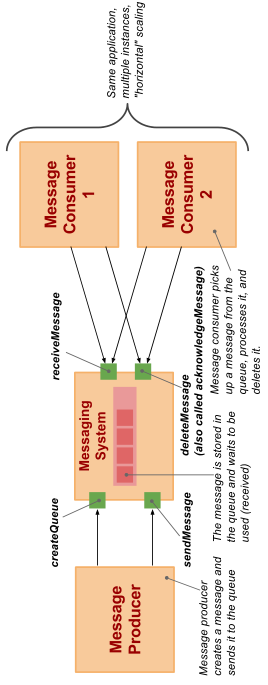
\includegraphics[width=1.2\textwidth]{obr/vitvar_mq.png}
 	\caption[Příklad MQ systému s producentem zpráv a konzumenty]{Příklad MQ systému s producentem zpráv a konzumenty. Zdroj: \cite{vitvarMq}}\label{fig:vitvarMq}
\end{figure}	

Recommeng systém bude taktéž komunikovat s databází kvůli nutnosti průběžného ukládání informací o stavu, respektive kvůli možnosti načíst poslední uložený stav při novém startu aplikace.

Veškerá data pro výpočet a predikci budou jinak udržována přímo ve vnitřní paměti (uvnitř JVM).

\subsubsection{Klient}

Klientská strana není nikterak složitá. Potenciální uživatel aplikace má v zásadě dvě možnosti, jak s platformou komunikovat:

\begin{itemize}
	\item Jen a pouze zasíláním žádostí na REST API.
	\item Kombinací zasílání žádostí na REST API společně s přímou komunikací s Recommeng systémem prostřednictvím fronty zpráv.
\end{itemize}

Některé ze systémových funkcionalit nelze bez komunikace s REST API využívat. Do této kategorie spadá například přidání nového vztahu k položce ve fulltextovém indexu nebo zaslání žádosti o doporučení obsahu některým z podporovaných algoritmů. 

Přímé spojení s platformou skrze frontu zpráv bez nutnosti zapojení prostředníka v podobě REST API by ale měly umožňovat všechny možnosti použití Recommeng systému. Jmenovitě jde především o vytváření kolekcí se seznamem algoritmů, dále zasílání žádostí o radu pro výběr algoritmu a též metody informující systém o uživatelově chování jako zvolení konkrétního algoritmu nebo zaslání zpětné vazby o doporučení. 

V diagramu~\ref{fig:recommeng} jsem se snažil zachytit různé formy komunikace klienta se systémem. Pro lepší názornost jsou jednotlivé žádosti barevně odlišeny. Ty lze považovat za modelové případy užití inspirované systémovými požadavky.

\paragraph{Zaslání zpětné vazby k doporučené položce}
\emph{Pozn.} V diagramu~\ref{fig:recommeng} je klient odlišen červenou barvou. 

Jedná se o klienta přidávajícího nový vztah mezi položkou a jejím uživatelem do úložiště.

\begin{itemize}
	\item klient zašle žádost na rozhraní
	\item aplikace (Web Application 1) za rozhraním se spojí s indexem
	\item v případě zdárného průběhu se přidá do indexu informace o tom, že 1 uživatel dělá něco s 1 dokumentem
	\item klient obdrží odpověď s výsledkem žádosti
\end{itemize}

\paragraph{Žádost o radu při výběru metody pro doporučení obsahu}
\label{subsub:purple}

\emph{Pozn.} V diagramu~\ref{fig:recommeng} je klient odlišen fialovou barvou.

V diagramu je znázorněna situace, kdy klient zasílá platformě zpětnou vazbu ohledně doporučení, které dostal. Tato varianta může ale též představovat situaci, kdy klient žádá systém o radu, kterou metodou si má nechat doporučit obsah ve své budoucí žádosti o doporučení (viz varianta~\ref{subsub:yellow}).

\begin{itemize}
	\item klient zašle žádost na rozhraní
	\item aplikace (Web Application 1) za rozhraním se pokusí přistoupit k frontě zpráv
	\item pokud fronta existuje, žádost je přidána do fronty pro zpracování konzumentem (Recommeng systém)
	\item konzument zpracuje žádost a zasílá odpověď, kterou systém zpráv předá zpět do aplikace
	\item klient obdrží odpověď s výsledkem žádosti
\end{itemize}

\paragraph{Žádost o doporučení konkrétním algoritmem}
\label{subsub:yellow}

\emph{Pozn.} V diagramu~\ref{fig:recommeng} je klient odlišen žlutou barvou.

Situace znázorňuje situaci, kdy klient poptává doporučení obsahu konkrétním algoritmem. Toto doporučení klient poptává na základě odpovědi na žádost, která mu byla udělena systém (viz varianta~\ref{subsub:purple})). 

\begin{itemize}
	\item klient zašle žádost na rozhraní
	\item aplikace (Web Application 1) za rozhraním zvolí vybraný algoritmus pro doporučení
	\item algoritmus přistoupí k datům v indexu, nad kterými se provede doporučení
	\item klient obdrží odpověď s výsledkem žádosti
\end{itemize}

\paragraph{Komunikace bez využití RESTful API}

\emph{Pozn.} V diagramu~\ref{fig:recommeng} je klient odlišen modrou barvou.

Tento klient se rozhodl nevyužít možnosti komunikovat prostřednictvím REST API. Svou žádost zasílá přímo do fronty zpráv.

\begin{itemize}
	\item klient zašle žádost do fronty
	\item pokud fronta existuje, žádost je přidána do fronty pro zpracování konzumentem (aplikace Recommeng)
	\item konzument zpracuje žádost a zasílá klientovi odpověď
\end{itemize}

\subsection{Obecný návrh rozhraní}
\label{sec:recommeng}

\subsubsection{Rozhraní REST}
Dle zadání má platforma poskytovat API pro interakci se systémem a daty formou RESTful (HTTP implementace REST~\ref{rest}). Každý uživatel tak bude moci interagovat s rozhraním prostřednictvím zveřejněných endpointů.

Z prováděné analýzy vyplynuly požadavky na aplikační rozhraní takové, že je lze rozdělit do tří skupin dle podstaty úkolu, který mají plnit. 

\begin{itemize}
	\item Ensemble alias Recommeng systém
	\item Algorithms
	\item Articles
\end{itemize}

Návrh tříd na zjednodušených\footnote{Pro větší srozumitelnost neuvádím v parametrech metod typy, ale spíše sémantické významy parametrů. Není též přítomna spousta dalších, s uvedenými třídami spolupracujících tříd.} diagramech~\ref{fig:recommengRestNavrh} a~\ref{fig:recommengRestNavrh2} ilustruje metody běžícím za poskytovaným API.

V případě prvního diagramu~\ref{fig:recommengRestNavrh} jsou prostřednictvím API metod volány metody třídy \textbf{EnsembleZeroMqHelper}, která bude realizovat spojení s frontou zpráv Recommeng systému (třída \textbf{AsynchronousServer} na diagramu~\ref{fig:recommengNavrh}).

Druhým zjednodušeným diagramem~\ref{fig:recommengRestNavrh2} si lze utvořit představu o způsobu komunikace metod pro RESTful API se serverem Apache Solr (třída \textbf{SolrService}) a dále s jednotlivými doporučovacícmi algoritmy (skrze API \textbf{IAlgorithm}).

\begin{figure}\centering
	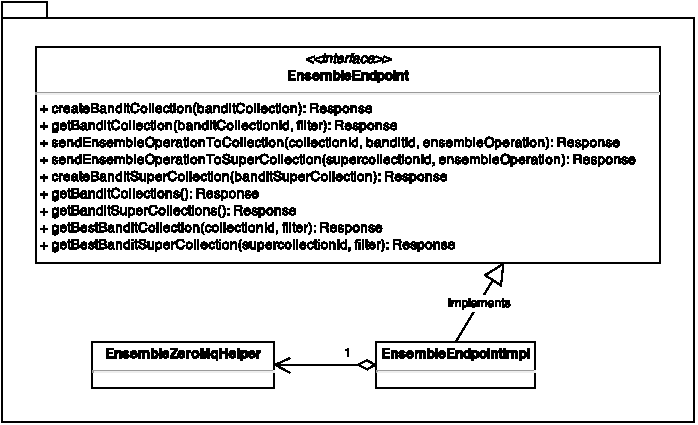
\includegraphics[width=1.0\textwidth]{obr/rest1.pdf}
 	\caption[Zjednodušený návrh tříd pro RESTful API endpoint pro komunikaci s Recommeng systémem.]{Zjednodušený návrh tříd pro RESTful API endpoint pro komunikaci s Recommeng systémem.}\label{fig:recommengRestNavrh}
\end{figure}	

\begin{figure}\centering
	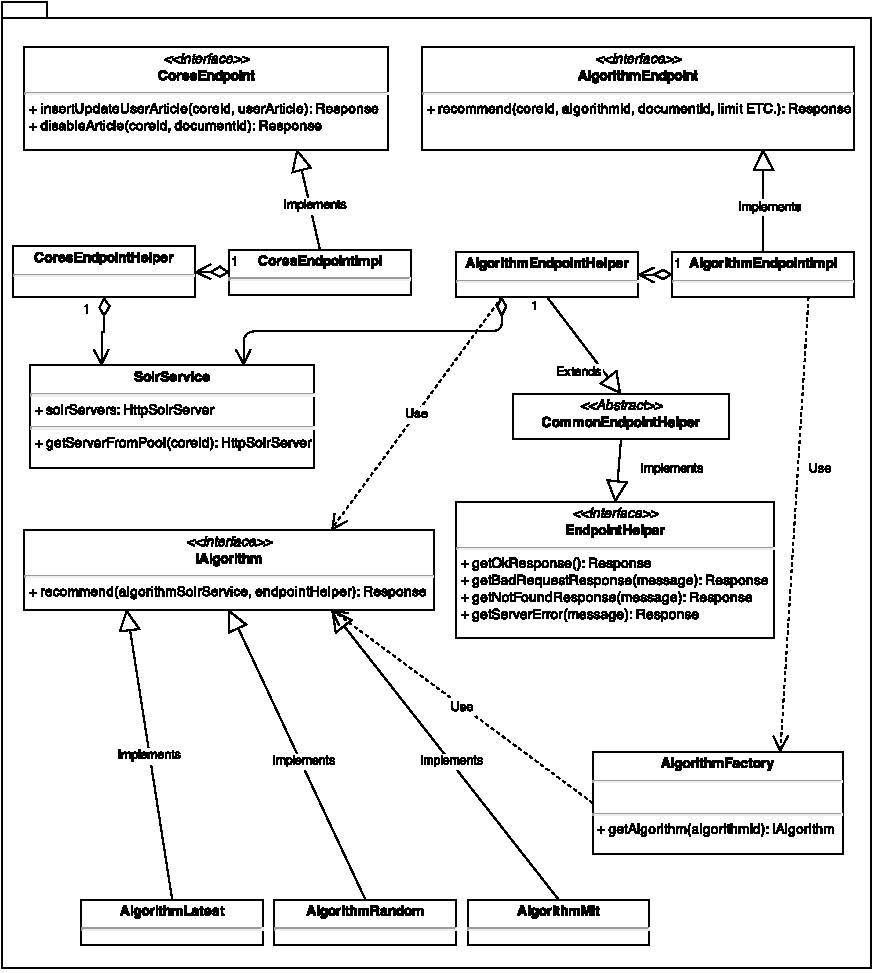
\includegraphics[width=1.0\textwidth]{obr/rest2.pdf}
 	\caption[Zjednodušený návrh tříd pro RESTful API endpointy pro komunikaci s jádrem Solr a s doporučovacími algoritmy.]{Zjednodušený návrh tříd pro RESTful API endpointy pro komunikaci s jádrem Solr a s doporučovacími algoritmy.}\label{fig:recommengRestNavrh2}
\end{figure}	

Z hlediska pohledu na část zdrojů je k dispozici diagram~\ref{fig:rest}, který by měl celou věc pomoct osvětlit. 

\begin{figure}\centering
	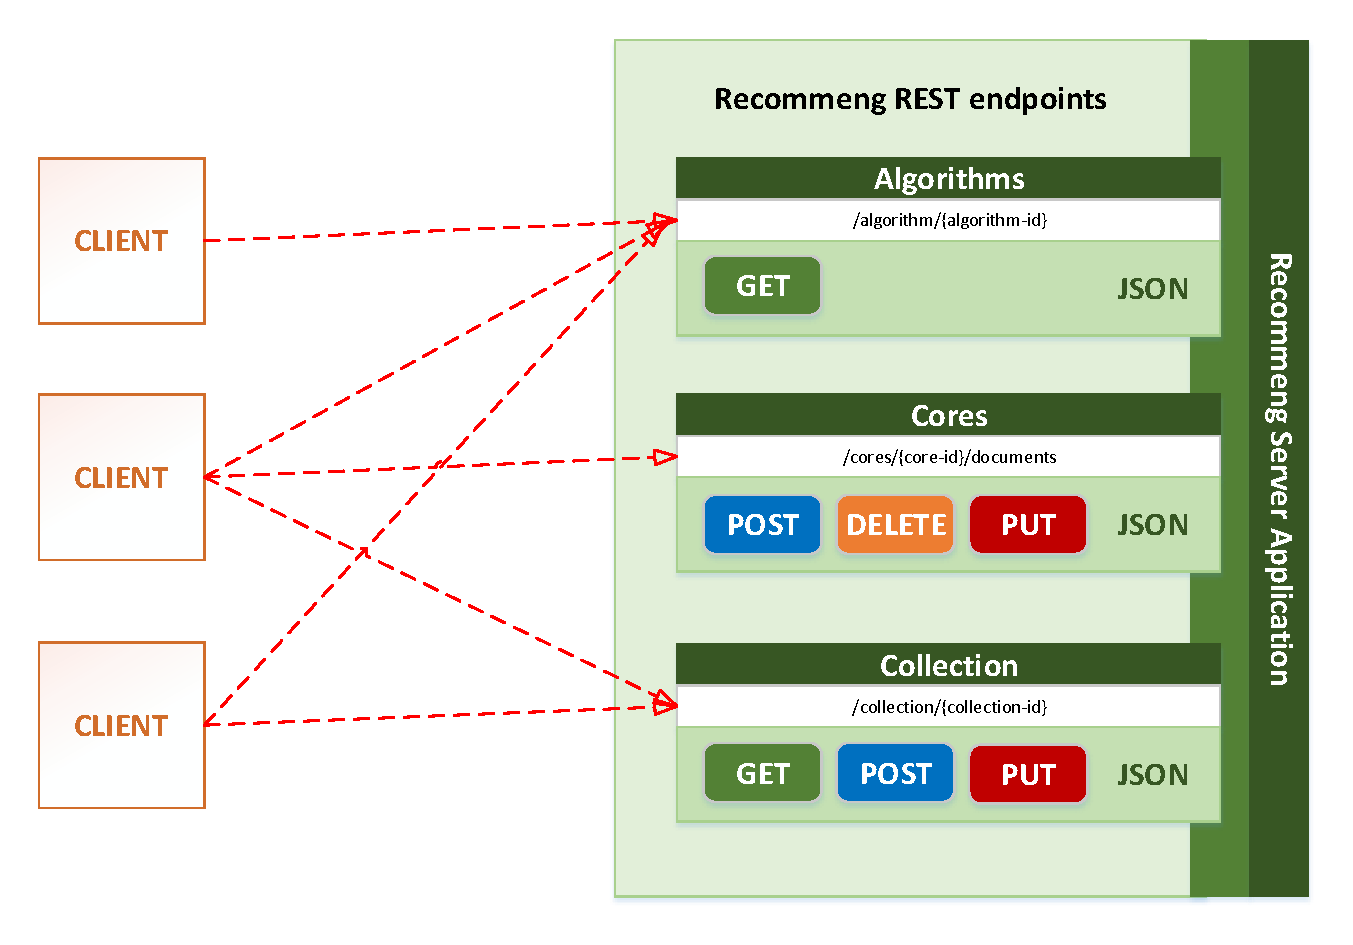
\includegraphics[width=1.0\textwidth]{obr/DIPLOMKA_rest.pdf}
 	\caption[Ukázka některých REST endpointů navrhovaného adaptibilního systému]{Ukázka některých REST endpointů navrhovaného adaptibilního systému}\label{fig:rest}
\end{figure}	

\paragraph{Ensemble}
Komunikace s rozhraním by měla umožňovat vytvářet v Recommeng aplikaci kolekce s identifikátory algoritmů a kolekce složené z těchto kolekcí (dále je budu označovat jako super kolekce), jenž budou zapojeny do kombinování a predikce. 

K tomu účelu budou sloužit endpointy:

\begin{verbatim}
	/collection
\end{verbatim}

\begin{verbatim}
	/supercollection
\end{verbatim}

Pokud uživatel zašle metodou POST žádost na tyto endpointy (obsahující jméno kolekce a seznam příslušných položek v těle požadavku), v případě dosavadní neexistence v systému budou kolekce vytvořeny a připraveny k užití systémem.

Dále by měla existovat možnost zaslat na kolekci či super kolekci prosbu o predikci nejlepšího jejího algoritmu pro doporučení.

\begin{verbatim}
	/collection/{collection-id}
\end{verbatim}

\begin{verbatim}
	/supercollection/{collection-id}
\end{verbatim}

Toho dosáhneme žádostí metodou GET, uvedením identifikátoru kolekce a případným specifikováním požadovaného výstupu (zda chceme vrátit jen nejlepší možnost či více možností seřazených sestupně od nejlepšího) v parametru dotazu.

Žádostí metodou GET bez specifikace ID bude navrácen seznam existujících kolekcí a super kolekcí v systému (existují-li v něm nějaké).

Kvůli učení a vývoji znalostí systému je nezbytné mít možnost zaslat systému informaci o výběru konkrétního algoritmu a též zpětnou vazbu vyjadřující, jak byl žádající uživatel s navrhovanou variantou spokojen. Toho bude dosaženo zasláním žádosti metodou PUT s informacemi uvedenými v těle požadavku.

\paragraph{Rozhraní pro sadu základních algoritmů}

Bude se jednat o jednoduchý endpoint, který si při žádosti vystačí s metodou GET.

\begin{verbatim}
	/algorithms/{algorithm-id}
\end{verbatim}

Úkolem je zpracovat žádost uživatele o doporučení algoritmem, jehož identifikátor je uveden v cestě. 

Hledání doporučení bude provedeno nad dokumenty ze specifikovaného indexu (identifikátor indexu je nutno uvést). V parametrech dotazu lze specifikovat další vstupy pro doporučení jako limit vrácených výsledků, identifikátor pro doporučení článků z jedné skupiny a další.

\paragraph{Rozhraní pro úložiště dat}

Důležité rozhraní umožňující zaznamenat například chování uživatele vzhledem ke sledovaným položkám.

\begin{verbatim}
	/cores
\end{verbatim}

\begin{verbatim}
	/cores/{core-id}/documents
\end{verbatim}

Prostřednictvím metody POST budou zasílány veškeré informace o položkách (u článku např. identifikátor, text, skupina, datum publikace) a jejím uživateli (identifikátor), které mají být uloženy do fulltextového indexu. Druhou podporovanou metodou je metoda DELETE pro vyřazení položky z doporučování. Metoda je použita v žádosti na týž endpoint jako metoda POST, pouze je nutné v parametru dotazu specifikovat identifikátor článku (z toho důvodu, že identifikátorem článku může být cokoliv, například URL adresa).

Metody a endpointy uvedené výše se dají považovat za hrubý přehled budoucí funkcionality systému. Kompletní dokumentace navrženého REST API je k nahlédnutí v příloze~\ref{restfulapi} na konci práce.

\subsubsection{Rozhraní Recommeng systému}
Znázorňuje jej třídní diagram~\ref{fig:recommengNavrh}. V případě úspěšně navázaného spojení se systémem jsou pomocí pracovních vláken \textbf{ServerWorker} volány jednotlivé procedury systému. Tyto žádosti obsluhuje API \textbf{EnsembleApiFacade}.

Stejně jako v případě diagramů~\ref{fig:recommengRestNavrh} a~\ref{fig:recommengRestNavrh2} se jedná o zjednodušený návrh, kde chybí spousta dalších tříd zapojených do systému. Diagram slouží pouze k ilustraci metod rozhraní a jejich funkcí pro daný systém.

\begin{figure}\centering
	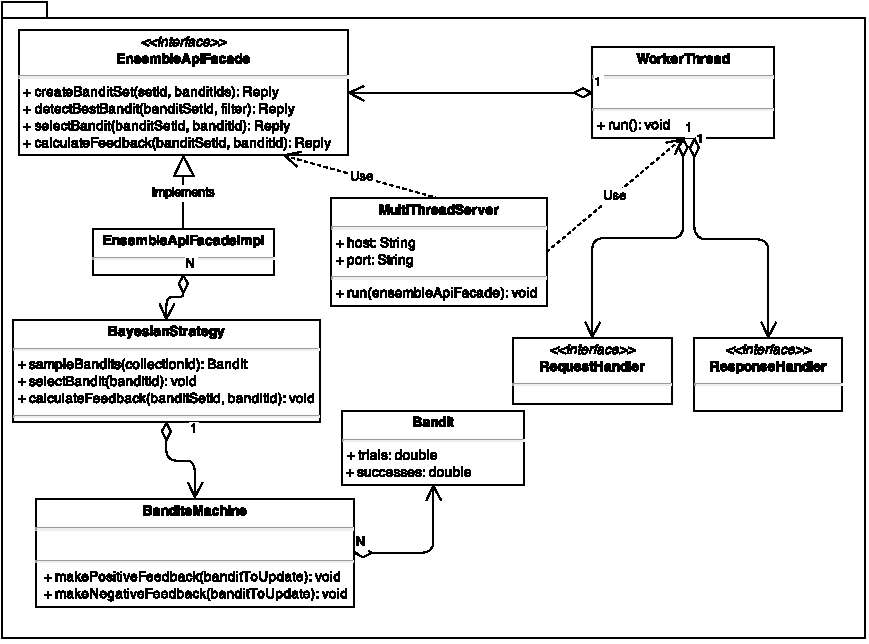
\includegraphics[width=1.0\textwidth]{obr/ensembleDiagram.pdf}
 	\caption[Zjednodušený návrh tříd v adaptibilním systému a ukázka API.]{Zjednodušený návrh tříd v adaptibilním systému a ukázka API.}\label{fig:recommengNavrh}
\end{figure}	

\subsubsection{Komunikace s frontou zpráv Recommeng systému}

Dle návrhu bude komunikace uživatele s Recommeng systémem, ať už komunikuje přímo či pomocí RESTful API, řešena prostřednictvím fronty zpráv.

Dalším úkolem tedy je navrhnout formát, jakým si budou vyměňovat producent s konzumentem data prostřednictvím volání vzdálených procedur Recommeng systému.

Vzhledem k obecné známosti protokolu HTTP jsem se rozhodl napodobit jeho chování a zachovat sémantiku:

\begin{itemize}
	\item metoda (method)
	\item cesta (path)
	\item tělo zprávy (body)
\end{itemize}

Podobně jako v HTTP, i v případě mnou navrhované komunikace bude na každou žádost ve tvaru \emph{method, path} a \emph{body} přicházet odpověď ve tvaru \emph{status} a \emph{body} s využitím různých návratových kódů pro stav (status). Všechny tyto informace budou ale prezentovány ve formátu JSON.
			
\subsection{Identifikace sady algoritmů}
Uživatel žádající o radu pro výběr nejlepšího algoritmu obdrží od systému identifikátor reprezentující tento algoritmus. 

Algoritmy pro doporučování vyhodnocují především informace o uživateli, položkách a hodnocení. Ukládány jsou ale i další údaje, například datum zveřejnění položky či její popis (u článku se může jednat o text zprávy). Také s těmito informacemi mohou doporučovací algoritmy pracovat. 

\subsubsection{Algoritmus náhodného výběru}

Jak je patrné již z názvu, tento algoritmus vybírá položky pro doporučení naprosto náhodným způsobem. Jeho hlavním úkolem je být zde pro srovnání s ostatními algoritmy. 

\subsubsection{Algoritmus výběru dle nejnovějších položek}

Doporučování dle nejnovějších položek je dalším z algoritmů s naivním přístupem k problému. Položky budou v tomto případě doporučovány sestupně dle zveřejněného data. 

\subsubsection{Algoritmus výběru nejlépe hodnocených položek}

Jedná se o první algoritmus založený na složitějším výpočtu. Položky vzešlé z doporučení budou dle určitých parametrů nějakým způsobem lepší než ostatní, které se v doporučení neobjevily. Takovým parametrem může být například hodnocení na škále od 1 do 5, počet pozitivních hodnocení, souhrnné číslo udávající počet přečtení článku nebo jiný z mnoha způsobů vyjádření zájmu o položku. 

\subsubsection{Algoritmus výběru dle podobnosti obsahu}

Algoritmus se snaží na základě podobnosti obsahu nalézt pro položku několik jí podobných položek z databáze. Podobnost se určuje porovnáním jednotlivých parametrů, například tagů, nadpisů nebo celého textu článku.

\subsubsection{Algoritmus kolaborativního filtrování}

Algoritmus je založen na modelu dřívějšího chování uživatele v systému. Model je většinou konstruován z chování většího množství uživatelů s podobným vkusem. V podstatě lze říci, že doporučení jsou založena na automatické spolupráci více uživatelů a výběru těch, kteří mají co nejpodobnější preference či chování.

Rozlišují se dva hlavní způsoby filtrování.

\paragraph{User-based}

\emph{``You may like it because your friends liked it.''}~\cite{cf}

Aneb filtrování založené na uživatelích. Jedná se o starší variantu kolaborativního filtrování. Podstatou je vzít na základě určité podobnosti skupinu uživatelů (zdroj~\cite{cf} udává cca 20 až 50) s podobných vkusem jako má uživatel, pro něhož je doporučení konstruováno, a poté předpovědět, jak moc zajímavá by pro uživatele byla pro něj dosud neznámá položka, se kterou jsou spojení uživatelé se stejným vkusem.

\paragraph{Item-based}

\emph{``You tend to like that item because you have liked those items.''}~\cite{cf}

Aneb filtrování založené na položkách, které použila v roce 2001 jako první společnost Amazon. Myšlenka je taková, že uživatel, který si v minulosti zakoupil nějakou položku, bude v budoucnu při dalším nákupu vyhledávat položku podobnou. Například předpověď toho, co si uživatel zakoupí v budoucnu, lze uskutečnit analýzou historie nákupů uživatele~\cite{itemcf}. 

\section{Principy a technologie}
\label{sec:sysanalys}

\subsection{RESTful API}
\label{rest}
\subsubsection{REST}
\textbf{REpresentational State Transfer (REST)} je architektonický styl definující určitá pravidla a vlastnosti návrhu API webových služeb orientovaných na zdroje. REST je silně založen na architektuře Klient-Server (server poskytuje přístup ke zdrojům, klient k nim může přistupovat a modifikovat je) a k jeho realizaci je možné využít protokolu HTTP (takovou realizaci pak nazýváme jako RESTful). Role tohoto protokolu zde není nikterak náhodná, neboť autorem REST není nikdo jiný než Roy Fielding, jenž je u protokolu HTTP podepsaný jako spoluautor~\cite{Fielding:2000:ASD:932295}. 

Díky protokolu HTTP lze následovat mnoho pravidel návrhu RESTful API, například přítomnost adresovatelných zdrojů, kdy je každý zdroj adresovatelný pomocí Uniform Resource Identifier (URI). RESTful pro manipulaci se svými zdroji používá též HTTP metody (GET, POST, PUT, DELETE, ale i další, například OPTIONS či PATCH). Další vlastností je užívání standardních stavových kódů\footnote{Definici všech stavových kódů viz \url{http://www.w3.org/Protocols/rfc2616/rfc2616-sec10.html}.} HTTP (typicky 2xx, 3xx, 4xx, 5xx) v odpovědi na žádost či bezestavová komunikace.

Data mohou být reprezentována v rozličných formátech jako XML, JSON či YAML.

\subsubsection{Jersey (JAX-RS)}
\textbf{Java API for RESTful Web Services (JAX-RS)}\footnote{https://jax-rs-spec.java.net} je standard definovaný v Java Specification Request 311\footnote{https://jcp.org/en/jsr/detail?id=311}. Jedná se o specifikaci pro RESTful webové služby implementované v programovacím jazyce Java.

Pomocí JAX-RS lze s využíváním anotací jednoduše a přehledně definovat sémantiku jednotlivých tříd a jejich metod z hlediska využití v architektuře REST. Příklady anotací jsou \emph{@Path(relativni\_cesta)} pro specifikaci relativní cesty zdroje, \emph{@GET} či \emph{@POST} specifikující typ žádosti nebo třeba \emph{@QueryParam} pro přiřazení parametru HTTP dotazu k hodnotě parametru příslušné metody třídy.

Pro účely implementace rozhraní systému Recommeng jsem zvolil vzhledem k předchozím zkušenostem referenční implementaci tohoto standardu v podobě frameworku \textbf{Jersey 2.x}. 

\subsubsection{JSON}
\textbf{JSON }\footnote{\url{http://www.json.org}} je jednoduchý a univerzální formát pro výměnu dat. Zkratka skrývá význam \emph{JavaScript Object Notation}. Jeho MIME (Internet media type) je application/json. V současné době se jedná o jeden z nejpoužívanějších formátů pro výměnu dat se službami REST. Výhodami jsou rychlost zpracování a snadnost použití.

Formát je postaven na dvou strukturách. 

\begin{description}
	\item \textbf{Array} je seřazený seznam hodnot, který je ohraničen závorkami
	\item \textbf{Object} je neseřazená kolekce dvojic klíč:hodnota ohraničený dvěma závorkami
\end{description}

Obě struktury lze do sebe zanořovat a vytvářet tak složitější struktury.

\subsection{Fronta zpráv a síťová komunikace}

\subsubsection{ØMQ}
\textbf{ØMQ (ZeroMQ)}\footnote{http://zeromq.org} je vysoce výkonná\footnote{Viz výkonnostní testy na oficiální stránce \url{http://zeromq.org/results:_start}.} síťová knihovna napsaná v programovacím jazyce C++ vhodná k nasazení v distribuovaných a vícevláknových aplikacích, které vyžadují velkou škálovatelnost. S jejím využitím lze poměrně snadno navrhnout komplexní komunikační systém. Ke komunikaci užívá socketů\footnote{Socket je mechanismus, kterým je možno zprostředkovat lokální čí vzdálenou komunikaci dvou uzlů, která má charakter klient/server~\cite{socket}.}. Duchovním otcem a spoluautorem knihovny je slovenský expert na oblast messaging middleware Martin Sústrik\footnote{\url{http://250bpm.com/contact}}.

Hned na úvod je nutné sdělit, že se nejedná o klasický messaging system (message-oriented middleware) takového typu, jakým je například Apache ActiveMQ\footnote{\url{http://activemq.apache.org}} a jemu podobné systémy. Takové systémy jsou většinou hotová řešení připravená k okamžitému nasazení a integraci s dalšími službami. 

Filosofie ZeroMQ je jiná, neboť jde především o multiplatformní knihovnu určenou k programovému využití (nabízí podporu více než 30 programovacích jazyků\footnote{TODO}). Pomocí jednoduchého socketového API umožňuje programátorovi sestavit si vlastní messaging system dle svého nejlepšího uvážen. Programátor využívá ze strany API veškerou podporu usnadňující práci se sítí a s trochou nadsázky lze prohlásit, že se stará pouze o zasílání zpráv. Sama socketová komunikace je výrazně zjednodušena.

Knihovna nám navíc dává kompletní svobodu v tom, jakým způsobem zakódujeme naši zprávu (JSON, BSON nebo jakýkoliv vlastní navržený formát).

Podporovány jsou čtyři protokoly pro komunikaci~\cite{zeromq1}:

\begin{description}
	\item[tcp] jako model síťově založeného přenosu (procesy na jedné síti)
	\item[inproc] jako model komunikace vláken uvnitř jednoho procesu
	\item[ipc] jako model komunikace mezi procesy (procesy out-of-box)
	\item[multicast]	komunikující skrze PGM\footnote{\url{http://tools.ietf.org/html/rfc3208}}.
\end{description}

Knihovna také definuje základní vzory zasílání zpráv, ať už se jedná o doručování zpráv na jednotlivé uzly, mapování uzlů na vlákna, procesy či umisťování zpráv do fronty\footnote{\url{http://zguide.zeromq.org/page:all\#Messaging-Patterns}}. Každý vzor zároveň určuje jinou síťovou topologii.

Základními vzory jsou:

\begin{itemize}
	\item Request-reply
	\item Pub-sub
	\item Pipeline		
	\item Exclusive pair
\end{itemize}

Nejvhodnějším vzorem pro mou práci je díky nátuře navrhovaného systému (zasílání zpráv a odpovědi na ně) vzor Request-reply, jehož konkrétní použití následuje záhy v sekci \nameref{sec:impl}. Ostatní vzory nemá smysl v rámci této práce popisovat.

Pro účely Recommeng systému jsem se rozhodl využít čistou Java implementaci knihovny ZeroMQ v podobě knihovny \textbf{jeroMQ}\footnote{\url{https://github.com/zeromq/jeromq}}. Z výkonnostního hlediska za původním řešením zaostává jen nepatrně\footnote{Viz srovnávací testy \url{https://github.com/zeromq/jeromq/wiki/Perfomance}.} a navíc je mnohem jednodušší integrovat ji do vyvíjené aplikace prostým přidáním knihovny do projektu.

\subsection{Úložiště dat}

\subsubsection{Apache Solr}
\textbf{Apache Solr}\footnote{\url{https://lucene.apache.org/solr}} je populární\footnote{Viz seznam serverů využívajících služeb Solr \url{https://wiki.apache.org/solr/PublicServers}} open-source platforma pro vyhledávání napsaná v programovacím jazyce Java. Jejími charakteristickými vlastnosti jsou podpora pro fulltextové vyhledávání, fasetové vyhledávání (analogie ke konstrukci GROUP BY v RDBMS), dobrá škálovatelnost pomocí kešování a distribuovaného vyhledávání, využívání vyhledávací konstrukce \emph{more like this}, o které bude řeč v sekci~\ref{sec:alg}, a také například tzv. \emph{near real-time indexing}\footnote{\url{https://cwiki.apache.org/confluence/display/solr/Near+Real+Time+Searching}} (dokumenty je možné vyhledávat téměř ihned po jejich zaindexování).

Z hlediska architektury programu jde o samostatný server pro fulltextové vyhledávání běžící v servletovém kontejneru (například Apache Tomcat). K indexaci a fulltextovému vyhledávání využívá ve svém jádru knihovnu Apache Lucene. 

\textbf{Apache Lucene}\footnote{\url{http://lucene.apache.org/core}} je vysoce výkonná knihovna pro účely vyhledávání v textu a indexování.

Vstupem pro indexaci jsou dokumenty. Každý takový dokument obsahuje množinu elementů, kde je tento element nazvaný jako \emph{field}). Každý field má své jméno, datový typ a případně další atributy.

Vstupem pro vyhledávání jsou textové řetězce (viz syntax\footnote{\url{http://lucene.apache.org/core/2_9_4/queryparsersyntax.html}}, případně dotazované objekty.

Index je uložen na disku ve formě souborů ve struktuře invertovaného indexu dokumentů~\cite{wiki:invindex}.

Ukázka definice několika field dokumentu ve schématu Solr:

\begin{lstlisting}[language=xml]
<field name="userId" type="int" indexed="true" stored="true" multiValued="true"/>	
<field name="time" type="date" indexed="true" stored="true"/>
\end{lstlisting}

Ukázka reprezentace dokumentu ve výsledku vyhledávání pomocí Apache Solr ve formátu XML:

\begin{lstlisting}[language=xml]
<doc>
   <int name="id">1</int>
   <str name="articleId">http://somedomain.org/somearticle.html</str>
   <str name="articleText">Hello Bob and Alice!</str>
   <int name="group">123</int>
   <long name="_version_">1465487644804775936</long>      
</doc>
\end{lstlisting}

Formu jejich spolupráce lze popsat tak, že Apache Solr poskytuje pro vyhledávání RESTful API, za kterým je skryto a voláno JAVA API knihovny Lucene. Díky tomu je možné pomocí protokolu HTTP komunikovat s Apache Solr z jakékoliv platformy napsané v jakémkoliv programovacím jazyce. 

K integraci Apache Solr s dalšími aplikacemi je možné vybírat ze spousty nástrojů a knihoven\footnote{\url{http://wiki.apache.org/solr/IntegratingSolr}}. Pro účely mé aplikace psané v programovacím jazyce Java jsem zvolil knihovnu \textbf{SolrJ}\footnote{\url{http://wiki.apache.org/solr/Solrj}} s klientským rozhraním pro vyhledávání, přidávání a aktualizaci indexu. 

\subsubsection{Apache Cassandra 2.0}
\textbf{Apache Cassandra 2.0}\footnote{\url{http://cassandra.apache.org}} je open-source distribuovaný DBMS navržený pro obsluhu velkého množství dat. Z hlediska datového modelu je Cassandra jakýmsi hybridem mezi key-value (pod 1 klíčem je uložena 1 hodnota) a column-oriented databázemi. V dokumentaci~\cite{cassdoc} se lze dočíst, že jde o row-oriented databázi.

Základem modelu je \emph{column family} (analogie tabulky v RDBMS), jež je složena z řádků a sloupců. Každý řádek má unikátní identifikátor ve formě klíče – každý řádek obsahuje více sloupců. Sloupce mají jméno, hodnotu a časovou značku. Výhodou proti RDBMS přístupu je to, že rozdílné řádky ze stejné column family nemusí sdílet stejnou množinu sloupců – do jedné nebo více řádek lze v libovolný čas zapsat jakýkoliv sloupec.

Vzhledem k tomu, že jedním z vyzdvihovaných případů užití databáze je uchovávání časových snímků, rozhodl jsem se ji experimentálně zapojit do vytvářeného Recommeng systému. Ještě předtím jsem však detailněji zkoumal možnost použití jiné NoSQL databáze, a to \textbf{Redis}. 

Redis je klasickou key-value databází uchovávající data primárně v paměti. Postupným vývojem se jeho funkcionalita propracovala k tomu, že pod jeden klíč je nyní možné uložit několik datových struktur (např. množiny a asociativní pole). Vzhledem k ukládání dat do paměti disponuje značnou rychlostí, navíc jej lze dle konfigurace nastavit tak, aby se obsah paměti průběžně ukládal na disk pro potřeby snadného obnovení dat v případě pádu aplikace.

Jeho zapojení do aplikace jsem zvažoval ve fázi zkoumání, jakým způsobem bude v adaptibilním systému řešen failover dat. Po následném návrhu datového modelu pro ukládání časových snímků stavu aplikace jsem však sáhl po použití Apache Cassandra jako po lepší z nabízených variant pro budoucí potřeby práce (rozsahové dotazy, vizualizace vývoje systému apod.). 

Velkým benefitem je podpora Cassandra Query Language (CQL), dotazovacího jazyka umožňujícího vytvářet podobné konstrukty, jaké nabízí jazyk SQL. CQL je nyní k dispozici ve verzi 3.1 a s pomocí \textbf{DataStax Java Driver 2.0} mohu snadno manipulovat s databází přímo ze své aplikace. 

\subsection{Ostatní použité technologie}

\subsubsection{Apache Mahout}
\label{mahout}
\textbf{Apache Mahout}\footnote{\url{https://mahout.apache.org}} je knihovna napsaná v programovacím jazyce Java, jež poskytuje implementaci rozličných technik z oblasti strojového učení:

\begin{itemize}
	\item \textbf{shlukování (clustering)} – položky nacházejících se v určitých třídách (například webové stránky či novinové články) jsou organizovány do skupin tak, že položky nacházející se v těchto skupinách jsou si vzájemně podobné
	\item \textbf{klasifikace (classification)} – učení se ze stávajících kategorizací a zařazování neklasifikovaných položek do nejvhodnější kategorie
	\item \textbf{doporučování (recommendation)}
	\item \textbf{často se vyskytující skupiny položek (frequent itemset mining)} – analýza položek v rámci nějaké skupiny (například nákupní košík) a identifikace, které položky se nejčastěji vyskytují pohromadě
\end{itemize}

Pro tyto techniky realizuje příslušné algoritmy jako například kolaborativní filtrování, k-means, náhodné lesy, skryté markovské modely a další. Některé algoritmy jsou připraveny pro běh v distribuovaném módu s využitím paradigmatu Map/Reduce, některé pak v lokálním módu (samotný Mahout je založen na Apache Hadoop, ale lze jej pohodlně využívat i bez něj)~\cite{mahouttut}. Mahout poskytuje též knihovny pro obecné matematické operace (zaměřené hlavně na oblast statistiky) a kolekce\footnote{\url{https://mahout.apache.org/users/basics/mahout-collections.html}}. 

Využít jej pro potřeby své práce jsem se rozhodl poté, co jsem na něj narazil v projektu Mendeley~\ref{mendeley} během zkoumání existujících řešení doporučovacích systémů. 

\subsubsection{Spring Framework}
Při tvorbě každého nového Java projektu od základu je dobré zamyslet se nad možností využít některý z mnoha frameworků a dalších užitečných nástrojů, s jejichž pomocí si lze do značné míry usnadnit proces vývoje. Díky dobrým zkušenostem z dřívějších projektů jsem zvolil open-source framework pro tvorbu moderních enterprise aplikací \textbf{Spring}\footnote{\url{http://projects.spring.io/spring-framework}}. 

Jeho výhodami jsou snadná konfigurovatelnost, podpora dependency injection, rozšiřitelnost a také integrace s jinými frameworky. V mém případě to byla integrace s frameworkem Jersey, kterou jsem využil při implementaci RESTful API.

\subsubsection{Apache Tomcat}
\textbf{Apache Tomcat} je známý open-source webový server a servletový kontejner. Jedná se o oficiální referenční implementaci technologií Java Servlet a Java Server Pages (JSP). Na serveru mohou běžet uživatelské servlety (programy napsané v Javě), které umí zpracovávat požadavky zasílané pomocí HTTP protokolu a tímtéž protokolem na ně odpovídat. Apache Tomcat zde slouží jako zásobník servletů starající se o jejich spouštění, běh, ukončování a podobně.

\subsubsection{Správa závislostí}
Často slýchaným pojmem z úst mnoha vývojářů v programovacím jazyce Java je tzv. \emph{classpath hell}. V podstatě jde o problémy spojené s načítáním programových tříd. V dnešní době existuje spousta nástrojů schopných tento problém efektivně řešit používáním správně projektové struktury, sestavovacích nástrojů a nástrojů pro správu závislostí. Jmenujme například Apache Ant společně s Apache Ivy, Gradle nebo třeba Apache Maven.

\textbf{Apache Maven} jsem použil při implementaci všech komponent aplikace.

\section{Realizace doporučovací platformy}
\label{chap:impl}

Následující kapitola se zaměřuje na popis programátorských postupů, které jsem použil při implementaci systému.

\subsection{Recommeng systém}
\label{sec:impl}

Adaptibilní systém poběží na serveru jako samostatná \emph{Java Application} s názvem \textbf{Ensemble}.

\subsubsection{Zavedení systému}
Poté, co je aplikace spuštěna voláním metody \texttt{main()} třídy \textbf{EnsembleApp}, je v této metodě následně volána metoda \texttt{loadEnsembleApplication()} abstraktní rodičovské třídy \textbf{EnsembleAppBase}.

Metoda loadConsoleApplication() hraje roli zavaděče aplikace, neboť postupným voláním v sobě obsažených metod zavádí do provozu celý systém (vytvoření instance řídící třídy, napojení na databázi, inicializace API a spuštění asynchronního serveru). Hlavní řídící třídou aplikace je třída \textbf{ApplicationBean}. Jejím prostřednictvím je zavedena vrstva pro obsluhu zpráv i komponenty pro komunikaci s datovým úložištěm. Třída je zavedena z aplikačního kontextu frameworku Spring.

Ten je možné velice jednoduše konfigurovat pomocí anotací ve třídě \textbf{AppConfig}:

\begin{lstlisting}[language=java]
@Configuration
@EnableScheduling
@ComponentScan(basePackages = {
     "cz.cvut.bouchja1.ensemble.spring"
})
@PropertySource("classpath:application.properties")
public class AppConfig {
...
\end{lstlisting}

Anotace \emph{@EnableScheduling} a \emph{@ComponentScan} využijeme pro pravidelné ukládání stavu aplikace~\ref{task}, anotaci \emph{@PropertySource} zase pro možnosti parametrizace systému~\ref{param}.

\subsubsection{Parametrizace}
\label{param}
Pro účely experimentování se systémem, volbu databázového úložiště a testování funkčnosti s různě volenou konfigurací je nutné načítat konfiguraci z editovatelného \emph{properties} souboru. K tomu jsem využil Spring bean \textbf{PropertySourcesPlaceholderConfigurer}.

Konkrétní načítání v programu je pak velice jednoduché:

\begin{lstlisting}[language=java]
this.rate = Double.parseDouble(env.getProperty("ensemble.machine.rate"));
this.possitiveFeedback = Double.parseDouble(env.getProperty("ensemble.feedback.possitive.winner"));
this.possitiveFeedbackOthers = Double.parseDouble(env.getProperty("ensemble.feedback.possitive.losers"));
this.negativeFeedback = Double.parseDouble(env.getProperty("ensemble.feedback.negative.stupid"));
\end{lstlisting}

\subsubsection{Vrstva pro obsluhu zpráv}
\label{sub:messvrs}
Následující text popisuje postup, jakým jsem realizoval vrstvu pro obsluhu zpráv pomocí síťové knihovny ZeroMQ.

Většinová funkcionalita je řešena třídou \texttt{AsynchronousServer} (obsahující též vnitřní třídu \textbf{ServerWorker}) v programovém balíčku:

\begin{verbatim}
   cz.cvut.fit.bouchja1.ensemble.socket
\end{verbatim}

Postup tvorby by se dal shrnout do tří kroků:

\begin{enumerate}
	\item rozhodnutí o komunikačním protokolu
	\item definice síťové infrastruktury
	\item realizace vzoru pro zasílání asynchronních zpráv REQ/REP
\end{enumerate}

\paragraph{Rozhodnutí o komunikačním protokolu}
\label{subsub:kompr}
V prvním kroku bylo nutné rozhodnout o tom, jakým způsobem bude probíhat přenos dat směrem k Recommeng systému a naopak. Ze čtyř protokolů, jimiž disponuje ZeroMQ, jsem pro přenos dat zvolil síťový protokol \textbf{TCP}, a to z toho důvodu, že dle návrhu architektury by měl adaptibilní systém naslouchat na serveru a uživatelé s ním mít možnost navazovat spojení zvenčí mimo server.

Mezi komunikujícími klienty a Recommeng aplikací na serveru jsou vytvářena jednotlivá spojení a data jsou z jednoho koncového bodu na druhý přenášena ve formě bajtů.

Díky ZeroMQ API stačí připravit kontext, socket a metodě \texttt{bind()} nastavit adresu serveru s příslušným portem. Sama metoda se pak postará o zbylou práci (vytvoření endpointu pro příjem jednotlivých spojení a navázání na socket).

\begin{lstlisting}[language=java]
ZContext ctx = new ZContext();
//  Frontend socket talks to clients over TCP
Socket frontend = ctx.createSocket(ZMQ.ROUTER);
frontend.bind("tcp://" + host + ":" + port);
\end{lstlisting}

\paragraph{Definice síťové infrastruktury}
\label{subsub:queue}
Propojení jednotlivých síťových komponent vychází z nativní povahy architektury Klient-Server. Server zastává roli stabilnější komponenty v síti, bude tedy přijímat spojení (viz ukázka s metodou \texttt{bind()} výše). Zároveň bude nutné umístit mezi server a připojující se klienty prostředníka, jehož úkolem obsluha všech žádostí na server a zasílání odpovědí zpět klientům.

V případě více připojených klientů bude ZeroMQ automaticky obstarávat obsluhu všech příchozích žádostí. 

\paragraph{Realizace vzoru pro zasílání zpráv REQ/REP}
Pro zasílání zpráv jsem nejprve zvolil obousměrně komunikující vzor \emph{Request Reply}. Toto paradigma je známé z většiny serverových typů\footnote{HTTP, POP či IMAP}. Klient používá vlastní socket typu \textbf{ZMQ.REQ} k inicializaci žádosti, kterou následně odesílá na server. Server též užívá vlastního socketu \textbf{ZMQ.REP} ke čtení příchozí žádosti, po které zasílá odpověď. 

Problém je, že vzor Request-Reply toho v základní variantě mnoho neumožňuje, proto bylo nutné umožnit asynchronní komunikaci implementací rozšíření v podobě socketů \textbf{ROUTER} a \textbf{DEALER} (dříve nazývány jako XREP a XREQ). 

Řešení spočívá ve vytvoření více pracovních vláken (\emph{workers}) souběžně řešících příchozí požadavky. Za tímto účelem je nutné vytvořit v serverovém vlákně socket typu DEALER, kterému přiřadíme komunikační protokol \emph{inproc://}.

Na serverové straně probíhá komunikace následovně: 

\begin{lstlisting}[language=java]
//  Frontend socket talks to clients over TCP
Socket frontend = ctx.createSocket(ZMQ.ROUTER);
frontend.bind("tcp://" + host + ":" + port);

//  Backend socket talks to workers over inproc
Socket backend = ctx.createSocket(ZMQ.DEALER);
backend.bind("inproc://backend");

//  Launch pool of worker threads, precise number is not critical
for (int threadNbr = 0; threadNbr < 5; threadNbr++) {
    new Thread(new ServerWorker(threadNbr, ctx, api, new RequestHandlerJson(), new ResponseHandlerJson())).start();
}

//  Connect backend to frontend via a proxy
ZMQ.proxy(frontend, backend, null);
\end{lstlisting}

Kvůli podpoře více TCP spojení utvářených vůči serveru je nutné předřadit před socket typu DEALER ještě další typ socketu, kterým je ROUTER (byl vidět již v ukázce~\ref{subsub:kompr}) hrající roli frontend socketu. 

ROUTER přiřazuje vnitřní identifikátor každému k němu se připojujícímu socketu a následně obdrženou zprávu předává dále prostřednictvím socketu typu DEALER (backend socket) na jedno ze svých pracovních vláken.

Pracovním vláknům jsou přes parametry předány instance třídy \textbf{RequestHandlerJson} a \textbf{ResponseHandlerJson()}, takže jsou schopny obsluhovat příchozí žádosti v tomto formátu.

O obsluhu požadavků a správnou komunikaci frontend socketů s backend sockety se stará \emph{ZMQ.proxy}, který hraje roli prostředníka zmíněného výše~\ref{subsub:queue}.

Pracovní vlákna (ServerWorker) používají též komunikační protokol inproc a socket typu DEALER.

\begin{lstlisting}[language=java]
Socket worker = ctx.createSocket(ZMQ.DEALER);
worker.connect("inproc://backend");
\end{lstlisting}

Komunikace probíhá tak, že DEALER komunikuje s DEALEREM. Oproti serverovému vláknu, který ale používal pro inproc spojení metodu \emph{bind()}, využívají pracovní vlákna metodu \emph{connect()}, čili se k němu připojují, přijímají zprávy a starají se o jejich vyřízení.

Po navázání spojení je v těle metody \emph{run()} pracovních vláken realizována veškerá komunikace s logikou systému. Dochází zde k předávání zpráv jednotlivým metodám systémového API. Bližším popisem se zabývá~\ref{serverworker}. 

Obsloužené zprávy jsou poté zasílány zpět na serverové vlákno, které je přeposílá komunikujícím klientům

\begin{figure}\centering
	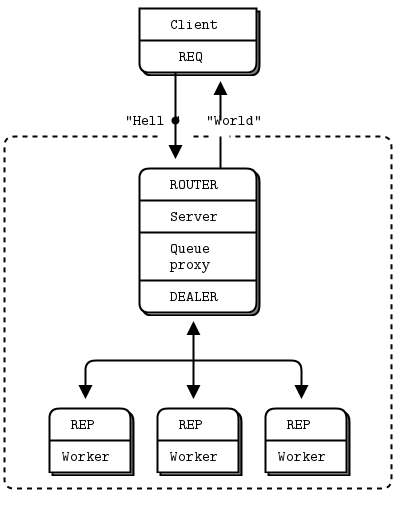
\includegraphics[width=0.8\textwidth]{obr/multithreadingServer.png}
 	\caption[Vícevláknový asynchronní server s využitím ROUTER a DEALER.]{Vícevláknový asynchronní server s využitím ROUTER a DEALER. Zdroj: \cite{mtserver}}\label{fig:mtserver}
\end{figure}	

Správnou synchronizaci vláken má na starosti již zmíněná ZMQ.proxy. To je jedna z pokročilých vlastností ZeroMQ – pro vývoj vícevláknových aplikací nejsou potřeba žádné mutexy, zámky, ani jakékoliv další formy komunikace~\cite{mtserver}.

\paragraph{Technika zasílání zpráv a ServerWorker}
\label{serverworker}
O několik řádku výše bylo vysvětleno, jakým způsobem jsou na serveru obsluhovány příchozí žádosti klientů. Nyní již víme, že tuto funkcionalitu mají na starosti pracovní vlákna typu \textbf{ServerWorker} a řekneme si, jakým způsobem jsou žádost zpracovávány.

Vláknová metoda \emph{run()} má na svědomí veškerou obsluhu žádosti. Každý jednotlivý \emph{worker} tak v sobě udržuje kontext komunikace a pokud je na vstupu validní žádost, pro její zpracování je vyvolána příslušná operace rozhraní systému Recommeng. Sestavená odpověď je zaslána zpět klientovi.

%\begin{verbatim}
\begin{lstlisting}[language=java]
try {
    Operation op = requestHandler.handleMessage(request);
    if (op.validateOperation()) {
        try {
            Reply reply = op.executeOperation(api);
            responseHandler.setReply(reply);
        } catch (Exception ex) {
            responseHandler.createInternalErrorReply("Internal error.");
        }
    } else {
        responseHandler.createErrorReply(op.getErrorMessage());
    }
} catch (MessageFormatException | IOException ex) {
    responseHandler.createErrorReply(ex.getMessage());
} catch (NullPointerException ex) {
    responseHandler.createErrorReply("Unrecognized operation.");
}
\end{lstlisting}

Výsledkem zpracování zprávy je operace. Spuštění vhodné operace je realizováno návrhovým vzorem Command. \textbf{Operation} je rozhraní deklarující metody pro validaci operace (\texttt{validateOperation()}) a její vykonání (\texttt{executeOperation()}).

Každá třída implementující toto rozhraní je pak konkrétní operací zasílanou na rozhraní systému. 

Všechny typy podporovaných operací se nacházejí v aplikaci Ensemble v balíčku:

\begin{verbatim}
   cz.cvut.fit.bouchja1.ensemble.operation
\end{verbatim}

Jedná se o třídy splňující funkcionalitu dle funkčních požadavků~\ref{sec:req}. Jsou jimi například:

\begin{itemize}
	\item \texttt{OperationCreateBanditCollection}
	\item \texttt{OperationCreateBanditSuperCollection}	
	\item \texttt{OperationDetectBestBandit}
	\item \texttt{OperationFeedbackSupercollectionBandit}
	\item \texttt{OperationUseSupercollectionBandit}			
\end{itemize}

Výsledkem vykonání operace je vždy odpověď (třída \textbf{Reply} obsahující stavový kód, tělo zprávy, případně další hodnoty jako seznam algoritmů apod.), která je pomocí třídy \textbf{ResponseHandlerDefault} prezentována zpět klientovi.

\subsubsection{API}
API systému Recommeng reprezentuje interface \textbf{EnsembleApiFacade}. Podporované metody jsou vidět na obrázku~\ref{fig:recommengNavrh}.

Tyto metody jsou volány prostřednictvím operací z vrstvy pro obsluhu zpráv~\ref{sub:messvrs}. Metody jsou přímo napojeny na bayesovské strategie, které jsou jedněmi ze stěžejních součástí systému.

Ukázkovou metodou je například metoda zprostředkovávající detekci nejlepšího algoritmu ze zadané kolekce. Nejprve proběhne ověření, zda v systému opravdu taková kolekce, vůči které je žádost směřována, existuje. Následně dojde k provedení žádosti a vytvoření odpovědi.

\begin{lstlisting}[language=java]
@Override
public Reply detectBestBandit(String banditCollectionId, String filter) {
    ResponseHandler responseHandler = new ResponseHandlerJson();
    Reply reply;

    if (existBanditSetId(banditCollectionId)) {
        BayesianStrategy strategyToUse = getStrategyByCollectionId(banditCollectionId);
        if ("best".equals(filter)) {
            Bandit banditToChoose = strategyToUse.sampleBandits();            
            responseHandler.createSuccessReplyDetection("You should choose bandit with name " + banditToChoose.getName() + " now. He is the best for this context.", banditToChoose.getId(), banditToChoose.getName(), strategyToUse.getId());
        } else {
            List<Bandit> banditsByOrder = strategyToUse.sampleBanditsAll(banditCollectionId);
            responseHandler.createSuccessReply("Bandit IDs by order: " + banditsByOrder.toString());
        }
        reply = responseHandler.returnReply();
    } else {
        responseHandler.createNotFoundReply("There is no collection with ID " + banditCollectionId + " in application.");
        reply = responseHandler.returnReply();
    }
    return reply;
}
\end{lstlisting}

Klient, který žádal systém o takovéto doporučení, obdrží zprávu ve tvaru:

\begin{lstlisting}
{"message":"You should choose bandit with name: latest. He is the best for this context.","status":200,"collection":1,"banditId":"latest","bestBandit":2}
\end{lstlisting}

Tento výstup lze použít jako parametry pro další dotaz (například pro zaslání zpětné vazby o zvolení algoritmu a posléze žádosti o doporučení obsahu navrácenou metodou).

\subsubsection{Bayesovská strategie pro kombinování metod}

Strategii mají na starosti třídy nacházející se v balíčku:

\begin{verbatim}
   cz.cvut.fit.bouchja1.ensemble.bandits
\end{verbatim}

\paragraph{Bandit}
Bandit je třída reprezentující jednoho konkrétní banditu. Každý bandita má svůj identifikátor a atributy pro zaznamenávání výher a pokusů během jednotlivých her. Ty reprezentují jeho dosavadní znalosti.
\paragraph{BanditsMachine}
BanditsMachine je třída reprezentující herní automat. Každá samostatná bayesovská strategie (BayesianStrategy) má právě jeden herní automat. Automat obsahuje seznam banditů a číselné konfigurace pro výpočty zpětné vazby a míry učení. Konfigurace se nastavuje ve vnějším soubor (viz~\ref{param}).
\paragraph{SuperBayesianStrategy} SuperBayesianStrategy je třída reprezentující super kolekci více bayesovských strategii. V případě přítomnosti dvou bayesovských strategií, například kontextových atributů \uv{ráno} a \uv{Evropa}, může z těchto strategií vytvořit super strategii \uv{ráno v Evropě}.
\paragraph{BayesianStrategy}	BayesianStrategy je třída reprezentující online učící strategii k řešení strategie Multi-Armed Bandit~\ref{sub:mabandit}. Vzhledem k přítomnosti super strategií je již jasné, že v systému může nezávisle na sobě fungovat více bayesovských strategií. 

\subsubsection{Důležité metody bayesovské strategie pro kombinování metod}
	Důležitou metodou třídy BayesianStrategy je metoda \texttt{sampleBandits()} starající se jednak o výběr z prior pravděpodobností distribucí banditů a následně o volbu nejlepšího z nich. Jedná se o implementaci teorie probírané v~\ref{bayes}.
	
\begin{lstlisting}[language=java]
public Bandit sampleBandits() {
    //sample from the bandits's priors, and select the largest sample
    for (Integer bandit : banditsMachine.getBanditList().keySet()) {
        BetaDistribution beta = new BetaDistribution(1 + banditsMachine.getBanditAtIndex(bandit).getSuccesses(), 1 + banditsMachine.getBanditAtIndex(bandit).getTrials() - banditsMachine.getBanditAtIndex(bandit).getSuccesses());
    double inverseDistribution = beta.inverseCumulativeProbability(Math.random());
    roundInverseDistributions.add(inverseDistribution);
    }
    int banditIndexChoice = MathUtil.argmax(roundInverseDistributions);
    roundInverseDistributions.clear();
    return banditsMachine.getBanditAtIndex(banditIndexChoice);
}
\end{lstlisting}	

Do rozdělení vstupují jako parametry dosavadní výsledky jednotlivých algoritmů z kolekce a dochází k výpočtu kvantilových funkcí~\ref{icdf} pro každý algoritmus, kdy je nakonec vybrán algoritmus s největší hodnotou a navrácen jako nejlepší možnost. 

Dalšími metodami jsou pak \emph{selectBandit(String banditId)} zpracovávající zpětnou vazbu o zvolení doporučeného algoritmu uživatelem a \emph{calculateFeedback(String banditCollectionId, String banditId, String feedbackValue)}. 

\begin{lstlisting}[language=java]
public void selectBandit(String banditId) {
    Bandit banditToUpdate = banditsMachine.getBanditAtIndex(Integer.parseInt(banditId));        
    banditsMachine.updateTrials(banditToUpdate);           
}

public void calculateFeedback(String banditCollectionId, String banditId, String feedbackValue) {
    Bandit banditToUpdate = banditsMachine.getBanditAtIndex(Integer.parseInt(banditId));
    banditsMachine.updateFeedback(banditToUpdate, feedbackValue);   
}  
\end{lstlisting}	

Těmito metodami je zajištěn přepočet hodnot, které si uchovávají jednotlivými algoritmy (trials, successes) jako svůj vnitřní stav vyjadřující dosud načerpané znalosti. Při každém přepočtu jsou tyto hodnoty ještě navíc násobeny konstantou určující míru učení~\ref{rate}.
    
V případě super strategie (třída SuperBayesianStrategy) je poměrně důležitou metodou \emph{chooseBestFromSuperStrategy()}. Ze zadané super kolekce je na základě odhadů vybrán vždy jeden nejlepší algoritmus z jejích kolekcí a pomocnou metodou \emph{bestBanditFromCombination(List<Bandit> banditsCombination)} je spočtena četnost výskytů jednotlivých algoritmů (navrácených jako nejlepší) z kolekcí. V případě shody stejného výskytu dvou a více algoritmů je na základě náhodného výběru zvolena jedna, která je doporučena uživateli.
    
\subsubsection{Zpětná vazba}
\label{implfeedback}     
Výše byly zmíněny dvě metody (selectBandit() a calculateFeedback()), které zprostředkovávají zpětnou vazbu pro systém. Nyní si pojďme popsat jejich realizaci.

Tělo metody updateTrials() je jednoduché a zpětná vazba týkající se připočítávání pokusů triviální:

\begin{lstlisting}[language=java]
double newTrials = rate * trials;
trials = newTrials + 1;
normalizedTrialsFrequencyInTime += totalTrialsCountsToBoost;
\end{lstlisting}	

V případě souhlasu s algoritmem, který rádce navrhuje, je k jeho vnitřnímu stavu uchovávající poměr pokusů (kolikrát byl vybrán) přičteno číslo 1.

Zajímavější je to v případě zasílání informace o kvalitě doporučení. Dle typu zpětné vazby (pozitivní či negativní) jsou volány dvě metody - makePositiveFeedback(banditToUpdate) či makeNegativeFeedback(banditToUpdate) a pomocí parametrů voleny tři hodnoty:

\begin{verbatim}
ensemble.feedback.possitive.winner=1.0
ensemble.feedback.possitive.losers=0.1
ensemble.feedback.negative.stupid=0.2
\end{verbatim}

V případě pozitivní zpětné vazby je danému algoritmu přičítána definovaná odměna (emph{result}):

\begin{lstlisting}[language=java]
double newSuccesses = rate * successes;
successes = newSuccesses + winner;
\end{lstlisting}	

Všem ostatním algoritmům je nějaká nadefinovaná hodnota v poměru odečtena (za předpokladu, že nemají vnitřní stav menší než poměrná odečítaná hodnota):

\begin{lstlisting}[language=java]
if (successes > (losers*rate)) {
    successes = successes - (losers*rate);
    double newSuccesses = rate * successes;
    successes = newSuccesses;
} else {
    double newSuccesses = rate * successes;
    successes = newSuccesses;            
}
\end{lstlisting}	

Tyto počty probíhají v případě pozitivní zpětné vazby. Ještě je nutné uvažovat případ, kdy dáme na radu systému, zvolíme algoritmus, který nám poradil, ale s výsledky doporučení nejsme spokojeni.V takovém případě je udělována negativní zpětná vazba. Negativní zpětná vazba je udělována pouze tomuto nevhodně zvolenému algoritmu. Vnitřní stav ostatních algoritmů zůstává nezměněn.

Penalizace je realizována následovně:

\begin{lstlisting}[language=java]
successes = successes - (stupid*rate);
double newSuccesses = rate * successes;
successes = newSuccesses;
\end{lstlisting}	
  
\subsubsection{Pravidelné ukládání časových snímků}
\label{task}
Pravidelné ukládání časových snímků jsem realizoval Spring démonem (\emph{cron}). Četnost jeho spouštění je možné volit přes parametr~\ref{param} v konfiguračním souboru aplikace. K tomuto účelu jsem vytvořil třídu \textbf{ScheduledJob} spouštějící pravidelný časový úkol, který zprostředkuje persistenci aktuálního stavu aplikace (tedy všech běžících bayesovských strategií), který je v té době v paměti, do databáze.

Samozřejmě za předpokladu, že je použití databáze v konfiguračním souboru nastaveno. V opačném případě by tovární metoda třídy \textbf{StorageFactory} zvolila k použití jinou formu práce s daty.

\begin{lstlisting}[language=java]
public static IStorage getStorage(Environment env) {
    switch (env.getProperty("storage")) {
        case "cassandra" : 
            return new CassandraStorage(env.getProperty("cassandra.host"), env.getProperty("cassandra.keyspace"));                
        default : 
            return new JvmStorage();
    }
}
\end{lstlisting}

Tento přístup vede k rozšiřitelnosti o další typy databází, které by mohl systém v budoucnu podporovat. 

\subsubsection{Spojení s databází}
Úložiště je realizováno třídou \textbf{CassandraStorage}. Během jejího zavádění do systému při startu aplikace jsou v konstruktoru volány dvě metody – \emph{connect()} a \emph{createSchema()}. V prvním případě dochází ke spojení s databázovým klastrem, pomocí kterého je následně získána \emph{session}.

Pomocí session a její metody \emph{execute()} lze vykonávat jednotlivé dotazy. 

Použita je hned v metodě createSchema(), která je zodpovědná za vytvoření datového modelu navrženého pro systém Recommeng.

Ukázka vytvoření keyspace pro všechny column families aplikace:

\begin{lstlisting}[language=java]
private void createSchema() {        
    session.execute("CREATE KEYSPACE IF NOT EXISTS " + keyspace + " WITH replication "
            + "= {'class':'SimpleStrategy', 'replication_factor':3};");
\end{lstlisting}

Column families jsem pro účely aplikace vytvořil tři – \emph{collection}, \emph{supercollection} a \emph{algorithm}.

Třída implementuje několik metod svého rozhraní IStorage pro uložení aktuálního stavu aplikace, načtení poslední známé konfigurace a vytvoření kolekcí banditů. Při realizaci funkcionality metod je bohatě využíváno možností, které nabízí DataStax driver pomocí CQL, například tvorba předpřipravených dotazů konstrukcí \textbf{PreparedStatement}. 

Následuje příklad ukládání aktuálního stavu z paměti systému do databáze.

\begin{lstlisting}[language=java]
@Override
public void saveCurrentState(LastEnsembleConfiguration strategies) {
    if (strategies != null) {
        for (BayesianStrategy strategy : strategies.getStrategies().values()) {
             Map<Integer, Bandit> bandits = strategy.getBanditsMachine().getBanditList();
            if (bandits.size() > 0) {
                PreparedStatement statement = session.prepare(
                        "INSERT INTO " + keyspace + ".algorithm "
                        + "(collection_id, algorithm_id, algorithm_name, event_time, trials_rate, successes_rate) "
                        + "VALUES (?, ?, ?, ?, ?, ?);");

                Date actualDate = Calendar.getInstance().getTime();

                for (Map.Entry<Integer, Bandit> entry : bandits.entrySet()) {
                    BoundStatement boundStatement = new BoundStatement(statement);
                    session.execute(boundStatement.bind(
                            strategy.getId(),
                            entry.getValue().getId(),
                            entry.getValue().getName(),
                            actualDate,
                            entry.getValue().getSuccesses()));
                    logger.info("Time: " + actualDate + "Saving bandit with ID " + entry.getValue().getName() + " into collection : " + strategy.getCollectionId());
                }
			...
			...			
}
\end{lstlisting}

\subsection{RESTful API}
\label{sub:restapi}

RESTful API je realizováno jako \emph{Java Web Application} s názvem \textbf{ensembleRestApi}.

Důležitou roli v modulu hraje přítomnost a správná konfigurace tzv. \emph{Web Application Deployment Descriptor} (soubor \textbf{/WEB-INF/web.xml}). V tomto souboru je definováno vše, co by měl server, na kterém aplikace poběží, o aplikaci vědět (informace o příslušných servletech, filtrech apod.).

Pro potřeby modulu RESTful API jsem v tomto souboru definoval \emph{listener\footnote{Listener je aplikace, jež vyčkává na vznik nějaké události. Jakmile událost nastane, listener zareaguje a převezme její řízení.} pro Spring}. Dále \emph{servlet pro Jersey}, jemuž jsem parametrem předal třídu \textbf{RecommengApplication}, a nastavil příslušné mapování servletu na specifickou URL.

\begin{lstlisting}[language=java]
<servlet>
    <servlet-name>jersey-serlvet</servlet-name>
    <servlet-class>
        org.glassfish.jersey.servlet.ServletContainer
    </servlet-class>
    <init-param>
        <param-name>javax.ws.rs.Application</param-name>
        <param-value>cz.cvut.fit.bouchja1.mi_dip.rest.client.service.RecommengApplication</param-value>            
    </init-param>        
    <load-on-startup>1</load-on-startup>
</servlet>

<servlet-mapping>
    <servlet-name>jersey-serlvet</servlet-name>
    <url-pattern>/*</url-pattern>
</servlet-mapping>
\end{lstlisting}

Pomocí třídy RecommengApplication, rozšiřující třídu ResourceConfig frameworku Jersey, jsem zaregistroval všechny aplikační komponenty, které budou použity JAX-RS aplikací, tedy vytvářeným RESTful API.

\begin{lstlisting}[language=java]
public RecommengApplication(){
    register(RequestContextFilter.class);
    register(AlgorithmEndpointImpl.class);
    register(ArticleEndpointImpl.class);
    register(EnsembleEndpointImpl.class);
    register(JacksonFeature.class);        
}
\end{lstlisting}

Třída registruje následující komponenty:

\begin{itemize}
	\item org.glassfish.jersey.server.spring.scope.RequestContextFilter
\end{itemize}
	Jedná se o Spring filter, který poskytuje propojení mezi JAX-RS a Spring žádostmi.

\begin{itemize}	
	\item cz.cvut.fit.bouchja1.mi\_dip.rest.client.endpoint.AlgorithmEndpointImpl
\end{itemize}	

\begin{itemize}
	\item cz.cvut.fit.bouchja1.mi\_dip.rest.client.endpoint.ArticleEndpointImpl
\end{itemize}	

\begin{itemize}
	\item cz.cvut.fit.bouchja1.mi\_dip.rest.client.endpoint.EnsembleEndpointImpl
\end{itemize}	

	Tyto tři třídy jsou služby REST API. 
	
\begin{itemize}	
	\item org.glassfish.jersey.jackson.JacksonFeature		
\end{itemize}	
	Registruje Jackson JSON poskytovatele pro zpracování příchozích dat ve formátu JSON.

Nakonec jsem definoval filtr \emph{CharacterEncodingFilter} s UTF-8 kódováním pro všechny URL splňující vzor:

\begin{lstlisting}[language=java]
<filter-mapping>
    <filter-name>CharacterEncodingFilter</filter-name>
    <url-pattern>/*</url-pattern>
</filter-mapping>    
\end{lstlisting}

\subsubsection{Realizace endpointů}
\label{sec:endpoints}
Třídy z balíčku:

\begin{verbatim}
cz.cvut.fit.bouchja1.mi_dip.rest.client.endpoint
\end{verbatim}

jsou služby typu REST obsluhující všechny žádosti směřující na jimi mapované zdroje. Programově má každá tato třída anotaci definující její relativní URI cestu. V případě třídy \textbf{ArticleEndpointImpl} vypadá definice následovně:

\begin{lstlisting}[language=java]
@Component
@Path(ArticleEndpointImpl.ENDPOINT_PATH)
public class ArticleEndpointImpl implements ArticleEndpoint {
    
    public static final String ENDPOINT_PATH = "/cores";
    public static final String USER_ARTICLE_PATH = "/{coreId}/document";

    @Autowired
    private ArticleEndpointHelper articleEndpointHelper;  	
    ...
\end{lstlisting}

Anotace \emph{@Path} v tomto případě značí, že třída se bude nacházet na URI \emph{/cores}.

Jedna z jejích služeb umožňující vytvářet či aktualizovat informace o zpětné vazbě u dokumentu v indexu (zasíláním žádostí na URI zdroje \emph{/cores/\{coreId\}/document}) je definována takto:

\begin{lstlisting}[language=java]
@Path(USER_ARTICLE_PATH)
@Consumes({MediaType.APPLICATION_JSON})
@Produces({MediaType.APPLICATION_JSON, MediaType.APPLICATION_XML})
@POST
@Override
public Response updateBehavioralToArticle(@PathParam("coreId") String coreId, UserArticleDocument userArticle) {
    return articleEndpointHelper.updateBehavioralToArticle(coreId, userArticle);
} 
\end{lstlisting}

O samotné reprezentaci zdroje referuje příslušná podpodsekce~\ref{subsub:resource}.

Provádění má na starosti v tomto případě \textbf{ArticleEndpointHelper}. Ostatní služby mají též své helpery – třídy pomáhající jim v obsluze žádosti zodpovědné za vytváření odpovědí, které rozšiřují rodičovskou třídu \textbf{CommonEndpointHelper} implementující rozhraní \textbf{EndpointHelper}.

Rozhraní deklaruje více metod souvisejících s odpovědí, například metody pro vytvoření odpovědi dle typu návratového kódu a sestavení odpovědi.

\begin{lstlisting}[language=java]
public Response getNotFoundResponse(String message);
public Response build(ResponseBuilder builder, String message);
\end{lstlisting}

Proces tvorby odpovědi pak vypadá tak, že konkrétní helper volá ve své metodě službu zajišťující komunikaci s indexem. V případě metody \emph{updateBehavioralToArticle(String coreId, UserArticleDocument userArticle)} pro vkládání vztahu uživatel-hodnocení-článek do indexu je po provedení příslušných kontrol, kterými jsou validace vstupních dat a podobně, vytvořena odpověď.

\begin{lstlisting}[language=java]
public Response updateBehavioralToArticle(String coreId, UserArticleDocument userArticle) {
    Response resp = null;
    if (solrService.isServerCoreFromPool(coreId)) {
        String message = UserArticleValidator.validateUserArticle(userArticle);
        if ("success".equals(message)) {
            try {
                solrService.putUserArticle(coreId, userArticle);
                resp = getOkResponse("User-rating-item succesfully added into Solr core.");
            } catch (SolrServerException ex) {
                logger.error(ex);
                resp = getServerError(ex.getMessage());
            } catch (IOException ex) {
                logger.error(ex);
                resp = getServerError(ex.getMessage());
            }
		...
		...
    return resp;
}
\end{lstlisting}

Helper tedy volá dle výsledků programu jednu z metod své rodičovské třídy (například \emph{getBadRequestResponse(message)}) s příslušnou zprávou v parametru. Metodou \emph{build(ResponseBuilder builder, String message)} je pak vytvářena samotná odpověď.

\begin{lstlisting}[language=java]
@Override
public Response getNotFoundResponse(String message) {
    return build(Response.status(Response.Status.NOT_FOUND), message);
}    

@Override
public Response build(ResponseBuilder builder, String message) {
    return builder.entity(message).build();
}
\end{lstlisting}

\subsubsection{Reprezentace zdrojů}
\label{subsub:resource}
Zdroje jsou jedním ze stěžejních konceptů architektury REST. Kromě toho, že jsou adresovány příslušnými globálními identifikátory (v HTTP realizaci např. pomocí URI), mají též jednu nebo více reprezentací, ve které jsou vystaveny okolnímu světu, a pomocí které je možné s těmito zdroji manipulovat. 

V modulu pro RESTful API reprezentuji zdroje jako třídy v Javě. Například při tvorbě zdroje \emph{/cores/{coreId}/document} je vytvářena třída \textbf{UserArticleDocument}. 

\begin{lstlisting}[language=java]
@XmlRootElement
public class UserArticleDocument implements Serializable {       
    
    private static final long serialVersionUID = -8039686696076337053L;    
    private String articleId;
    private int userId;    
    private double rating;
    private int groupId;
    ...
\end{lstlisting}

Reprezentace tohoto zdroje ve formátu JSON by pak mohla vypadat například takto:

\begin{lstlisting}
{
    "articleId":"http://somedomain.org/somearticle.html",
    "group":123,
    "userId":42,
    "userRating":5.0
}
\end{lstlisting}

\subsubsection{Komunikace s Recommeng systémem}
\label{sec:restrec}
Vytvořil jsem též službu \textbf{EnsembleEndpointImpl} pro komunikaci s Recommeng systémem. Rozdíl oproti zbylým dvou službám (AlgorithmEndpointImpl a ArticlesEndpointImpl) je v rozdílném chování a funkčnosti její pomocné třídy \textbf{EnsembleZeroMqHelper}.

Tato služba, ač běžící jako součást serverové aplikace, hraje vůči Recommeng systému roli klientskou. Pro vnější uživatele zastává tradiční roli serveru.

EnsembleZeroMqHelper zpracovává příchozí žádosti od uživatelů prostřednictvím RESTful API. Poté transformuje do JSON formátu žádost, kterou umí Recommeng systém zpracovat. 

\begin{lstlisting}[language=java]
EnsembleRequest req = new EnsembleRequest();
req.setMethod("POST");
req.setPath("/ensemble/services/collection");
req.setBody("collectionId=" + banditCollection.getName() + "&bandits=" + formatBanditIds(banditCollection.getBanditIds()));
\end{lstlisting}

Pro spojení se systémem je vytvořeno vlákno \textbf{ClientTask}, jemuž je parametrem předána zpráva ve formátu JSON, a které volá metodu \emph{call()}.

\begin{lstlisting}[language=java]
ExecutorService executor = Executors.newSingleThreadExecutor();
Future<String> result = executor.submit(new ClientTask(req.toString()));

try {
    resp = buildResponse(result.get());
} catch (Exception ex) {
    resp = getServerError(ex.getMessage());
}
\end{lstlisting}

V těle metody call se vytvoří klientský socket prostřednictvím tcp a předřazená žádost je odeslána do systému. ClientTask pak vyčkává na odpověď (\emph{resp}). Poté, co ji obdrží a zpracuje do formátu HTTP odpovědi (\emph{buildResponse()}), ji vrací zpět žádajícímu klientovi. 

\begin{lstlisting}[language=java]
ZContext ctx = new ZContext();
Socket client = ctx.createSocket(ZMQ.DEALER);
client.connect("tcp://localhost:5555");
\end{lstlisting}

\subsubsection{Komunikace sady algoritmů pro doporučování}
\label{sec:algcom}
Doporučení je vyvoláno klientskou žádostí na rozhraní reprezentované třídou \textbf{AlgorithmEndpointImpl} a její zpracování zajišťuje metoda \emph{recommend()}. Metoda má několik vstupních parametrů:

\begin{lstlisting}[language=java]
@Path(ALGORITHM_PATH)
@Produces({MediaType.APPLICATION_JSON, MediaType.APPLICATION_XML})
@GET
@Override
public Response recommend(@PathParam("coreId") String coreId,
        @PathParam("algorithmId") String algorithmId,
        @QueryParam(value = "groupId") int groupId,
        @QueryParam(value = "userId") int userId,
        @QueryParam(value = "documentId") String documentId,
        @QueryParam(value = "text") String text,
        @QueryParam(value = "limit") int limit) {
\end{lstlisting}

Jak vidno, metoda umí v žádosti přijmout spoustu parametrů. Při každém vyvolání jsou všechny existující příchozí parametry uloženy do mapy a ta je následně předána tovární metodě, jejímž cílem je vytvořit na základě uživatelského vstupu vhodnou instanci třídy pro doporučení obsahu.

\begin{lstlisting}[language=java]
Map<String, String> algorithmParams = createAlgorithmParams(coreId, algorithmId, groupId, userId, documentId, text, limit);
IAlgorithm algorithm = AlgorithmFactory.getAlgorithm(algorithmId, algorithmParams);

if (algorithm == null) {
    return algorithmEndpointHelper.createAlgorithmNotFound();
}
else return algorithmEndpointHelper.getRecommendation(algorithm);
\end{lstlisting}

Služby využívají pro zpracování žádostí a vytváření odpovědí pomocnou třídu \textbf{AlgorithmEndpointHelper} (podobně jako~\ref{sec:restrec}). Tato třída v sobě navíc udržuje odkaz v podobě instance třídy \textbf{SolrService}, kterou předává třídám implementující jednotlivé doporučovací algoritmy (viz dále v podsekci~\ref{sec:alg}). 

\paragraph{Třída SolrService}
	
Třída implementuje metody pro komunikaci s Apache Solr a funguje též jako pool instancí serverových spojení pro různá jádra Solr. Vytvoření poolu bylo nutností kvůli možnosti znovu použít již vytvořené instance třídy \textbf{HttpSolrServer}.

Jejími atributy jsou:

\begin{lstlisting}[language=java]
private String serverUrl;
private Map<String, HttpSolrServer> validServers = new HashMap<String, HttpSolrServer>();
private Set<String> validSolrCores;
\end{lstlisting}

HttpSolrServer je thread-safe\footnote{Programové operace jsou prováděny správně i tehdy, kdy jsou prováděny více vlákny současně.} a pokud jej použijeme k vytvoření nové instance s URL některého z jader Solr v parametru, je nutné tuto instanci znovu použít pro všechny žádosti směřující na danou URL~\cite{solrj}. 

V opačném případě, kdy jsou instance vytvářeny bez jakéhokoliv rozmyslu a strategie, hrozí \emph{leak} připojení~\cite{metawerx}.

Validní jádra Solr pro připojení do poolu se nastavují v souboru aplikačního kontextu pro Spring:

\begin{lstlisting}[language=xml]
<bean id="solrService" class="cz.cvut.fit.bouchja1.mi_dip.rest.client.solr.SolrService">
    <property name="serverUrl" value="http://localhost:8089/solr/"/>
    <property name="validSolrCores">
        <set>
            <value>mi_dip_core1</value>
            <value>mi_dip_core2</value>
        </set>
    </property>        
</bean>  
\end{lstlisting}

SolrService obsahuje také metodu \emph{createValidSolrServers()}, jež je anotována jako \emph{@PostConstruct}.

Metoda s anotací @PostConstruct je vyvolána ještě před samotným vytvořením instance třídy. Účelem je naplnění poolu příslušnými validními instancemi spojení.

\begin{lstlisting}[language=java]
Iterator<String> validCores = validSolrCores.iterator();
while (validCores.hasNext()) {
    String core = validCores.next();
    validServers.put(core, new HttpSolrServer(serverUrl + core));
}
\end{lstlisting}

Kdykoliv je pak metodách tříd doporučovacích algoritmů navazováno spojení se serverem, dle zadaného identifikátoru jádra (coreId) se bere instanci z poolu, který má parametry \emph{HashMap<String, HttpSolrServer>}. 

\begin{lstlisting}[language=java]
HttpSolrServer server = solrService.getServerFromPool(coreId);
\end{lstlisting}

\subsection{Algoritmy pro doporučování obsahu pomocí Apache Solr}
\label{sec:alg}
Třídami, které jsou schopné různými způsoby doporučovat obsah, jsou:

\begin{itemize}
	\item AlgorithmWeightedRating
	\item AlgorithmLatest
	\item AlgorithmMlt
	\item AlgorithmRandom
	\item AlgorithmUserBasedCf
	\item AlgorithmItemBasedCf				
\end{itemize}

Všechny tyto třídy implementují rozhraní IAlgorithm a veškerá logika doporučení je vykonávána v implementacích metody recommend() konkrétních doporučovacích tříd a jejich pomocných metod. 

\subsubsection{Reprezentace dokumentů pro účely doporučování}

Pro potřeby modelové úlohy bylo nutné zamyslet se nad reprezentací a strukturou dat v Apache Solr. Z požadavků a technických možností Solr vyplynulo přímočaré řešení spočívající ve vytvoření dvou jader - jedno pro vkládání a uchovávání článků (\emph{articleCore}), druhé pro zaznamenávání interakce uživatele s doporučenými články (\emph{behavioralCore}). 

Jádro pro články budou při svých doporučeních využívat obsahově založené algoritmy (random, latest, more like this), jádro pro interakce budou využívat algoritmy pracující s uživatelskými hodnoceními (nejlépe hodnocené, kolaborativní filtrování).

\paragraph{Article core}
Jakýkoliv nově vytvořený článek je zaslán do tohoto jádra a přidán jako dokument s následující strukturou:

\begin{lstlisting}[language=xml]
 <doc>
    <int name="id">1</int>
    <str name="articleId">http://pnjj5cr4f9 f500k9vld.org</str>
    <str name="articleText">695t5r2fgy something.</str>
    <int name="group">789</int>
    <date name="time">2012-09-19T09:42:12Z</date>
    <long name="_version_">1467289878138978304</long>
</doc>
\end{lstlisting}

\paragraph{Behavioral core}
Po každé uživatelské interakci se článkem je tato interakce přidána do jádra jako trojice userId, articleId a userId\_rating. Pokud dokument s požadovaným articleId není v jádře přítomen, je v něm vytvořen. Pokud přítomen je, proběhne pouze přidání dvojice userId a userId\_rating.

\begin{lstlisting}[language=xml]
<doc>
    <int name="id">6</int>
    <str name="articleId">http://pnjj5cr4f9 f500k9vld.org</str>
    <arr name="userId">
      <int>1</int>
      <int>40</int>      
      <int>15</int>      
    </arr>
    <int name="group">789</int>
    <float name="1_rating">5.0</float>
    <float name="40_rating">5.0</float>
    <float name="15_rating">5.0</float>        
    <float name="weightedRating">5.0</float>
    <long name="_version_">1467370760759672832</long>
</doc>
\end{lstlisting}

\subsubsection{Algoritmus náhodného výběru}
Náhodný výběr by neměl mít již z podstaty věci příliš složitou implementaci. Rozhodl jsem se proto využít možnosti, kterou nabízí Solr. Rou možností je přidání speciálního typu a pole tohoto typu do schématu\footnote{Soubor schema.xml popisující veškeré detaily o tom, které filedy může jádro indexu obsahovat, a jakým způsobem s nimi má být nakládáno při přidávání dokumentů do indexu či dotazování.} jádra. 

\begin{lstlisting}[language=xml]
<fieldType name="random" class="solr.RandomSortField" indexed="true" />
<dynamicField name="random_*" type="random" />
\end{lstlisting}

Pro dotaz je poté možné využít speciálního vstupu pro řazení výsledků. Solr podporuje parametrem \emph{sort} řazení dokumentů dle specifikovaného pole v indexu. Díky definici náhodného typu lze zaslat jako vstup pro řazení field \emph{random} s náhodným prefixem. Například:

\begin{verbatim}
q=*:*&sort=random_12939291%20desc
\end{verbatim}

Solr tímto způsobem vyhodnotí pořadí dokumentů dle jména náhodného pole a verze indexu. To tedy znamená, že pokaždé, kdy je použito stejného jména náhodného pole a toho samého indexu (který nebyl mezi dotazy změněn), jsou navráceny ty samé výsledky. Proto jsem byl nucen zanést do dotazu ještě další prvek náhody a to tak, že pro názvy pole využívám náhodného čísla v rozsahu 1 až maximální hodnota celočíselného datového typu.

Programová realizace je pak již triviální:

\begin{lstlisting}[language=java]
int random = generator.nextInt(Integer.MAX\_VALUE) + 1;
String sortOrder = "random\_" + random;
  
query.setSortField(sortOrder, SolrQuery.ORDER.desc);
\end{lstlisting}       

\subsubsection{Algoritmus výběru dle nejnovějších položek}
Logika řazení funguje stejně jako v případě náhodného výběru výše díky parametru \emph{sort}. S tím rozdílem, že vstupem pro parametr je pole \emph{time} uchovávající datum vytvoření článku.

\begin{lstlisting}[language=xml]
<date name="time">2012-09-19T09:42:12Z</date>
\end{lstlisting}

Navrácené dokumenty jsou tak řazeny dle této hodnoty.

\subsubsection{Algoritmus výběru nejlépe hodnocených položek}
Pro výběr nejlépe hodnocených položek je již zapotřebí použít sofistikovanějšího mechanismu. Nelze se spoléhat na celkovou sumu či aritmetický průměr. Pomocí takového přístupu by totiž například položka, která byla hodnocena tisíckrát se známkou 1 (z 5 možných) byla považována za lepší než například položka hodnocená stokrát, ale vždy se známkou 5.

Rozhodl jsem se použít podobný přístup, jaký využívá známá filmová databáze IMDB\footnote{\url{http://www.imdb.com/chart/top}}. 

K výpočtu váženého hodnocení je využito bayesovských odhadů. Výpočet je realizován pomocí následující formule:

\begin{center}
$W = \frac{Rv + Cm}{v + m}$
\end{center}

\begin{description}
	\item[W] značí výsledné vážené hodnocení
	\item[R] značí průměrné hodnocení položky
	\item[v] značí počet hodnotitelů položky
	\item[m] značí minimální počet hodnocení potřebných k objevení se ve výsledku (IMDB pro potřeby výskytu filmu v prvních 250 užívá konstatnty 250000)
	\item[C] značí průměr hodnocení všech položek (IMDB používá hodnotu 7.0)
\end{description}

Výpočet váženého hodnocení probíhá po přidání každé další uživatelské interakce do jádra behavioralCore. Přepočet je nutný, neboť do dokumentů přibývají uživatelé s novými hodnoceními, mění se tak počty a průměrné hodnoty vstupující do vzorce. Mechanismu přepočítávání je realizován v metodě třídy \textbf{SolrService}.

\begin{verbatim}
recalculateWeightedRating(SolrInputDocument sid)
\end{verbatim}

Pro výpočet jsou důležitá pole userId a userId\_rating daného dokumentu.

Navrácení seřazených výsledků pak zajišťuje třída \textbf{AlgorithmWeightedRating} a nejedná se o nic jiného, než o seřazení dle vstupního parametru \emph{weightedRating}. Stejně jako v předchozích dvou případech.

\subsubsection{Algoritmus výběru dle podobnosti obsahu}
K doporučování dokumentů obsahově podobných jiným dokumentům v indexu mi byly opět velmi nápomocné nativní mechanismy Apache Solr. Tentokrát je řeč o vyhledávací komponentně známé jako \emph{MoreLikeThis}\footnote{\url{https://wiki.apache.org/solr/MoreLikeThis}}.

Přístup spočívá v přidání request handleru do konfigurace jádra\footnote{Soubor solrconfig.xml.}.

\begin{lstlisting}[language=xml]
<requestHandler name="/mlt" class="solr.MoreLikeThisHandler">
</requestHandler>
\end{lstlisting}

Podobnost je pak počítána na základě jednoho nebo více specifikovaných polí v dotazu. Do handleru lze zasílat velký počet parametrů, například:

\begin{description}
	\item mlt.fl pro specifikaci pole, které má být použito k výpočtu podobnosti,
	\item mlt.mintf pro minimální frekvenci termů dokumentu,
	\item mlt.minwl pro minimální délku slova uvažovaného pro výpočet podobnosti.
\end{description}

Realizace tohoto mechanismu se nachází ve třídě \textbf{AlgorithmMlt}, kde jsem specifikoval parametry. 

\begin{lstlisting}[language=java]
SolrQuery query = new SolrQuery();
query.setRequestHandler("/" + MoreLikeThisParams.MLT);
query.set(MoreLikeThisParams.MATCH_INCLUDE, true);
query.set(MoreLikeThisParams.MIN_DOC_FREQ, 1);
query.set(MoreLikeThisParams.MIN_TERM_FREQ, 1);
query.set(MoreLikeThisParams.MIN_WORD_LEN, 1);
query.set(MoreLikeThisParams.BOOST, false);
query.set(MoreLikeThisParams.SIMILARITY_FIELDS, "articleText");
query.set(MoreLikeThisParams.MAX_QUERY_TERMS, 1000);
query.setRows(limitToQuery);
query.setQuery("articleId:" + document.getFieldValue("articleId"));
query.setFilterQueries("group:" + document.getFieldValue("group"));
\end{lstlisting}

Jako vstup pro porovnání slouží jeden dokument z jádra.

\subsubsection{Algoritmus kolaborativního filtrování}
Při provádění analýzy stávajících řešení pro doporučování jsem se dozvěděl o knihovně Apache Mahout~\ref{mahout}, kterou využívá pro své potřeby systém Mendeley~\ref{mahout}, načež jsem se rozhodl pro to ji vyzkoušet.

Řešení budu demonstrovat na user-based přístupu realizovaného třídou \textbf{AlgorithmUserBasedCf}.

Nejprve bylo nutné získat z úložiště seznam uživatelských ID a ID dokumentů, které tito uživatelé hodnotili a tato data uložit do kolekce FastByIDMap.

\begin{lstlisting}[language=java]
FastByIDMap<FastIDSet> userData = new FastByIDMap<FastIDSet>();
\end{lstlisting}

Každý uživatel byl poté přidán do kolekce a z této kolekce byl vytvořen datový model.

\begin{lstlisting}[language=java]
userData.put(userRelatedId, new FastIDSet(itemValues));
DataModel model = new GenericBooleanPrefDataModel(userData);
\end{lstlisting}

Po vytvoření datového modelu je již možné konstruovat doporučení. Na výběr je několik podobnostních metrik, například euklidovská vzdálenost, pearsonův korelační koeficient či log-likelihood. Vzhledem k použití booleovského modelu preferencí jsem zvolil LogLikelihoodSimilarity. Pro doporučení je ještě stanovena sousedská funkce (doporučované položky pro uživatele jsou počítány na základě podobnosti mezi uživatelem a uživateli nacházejícími se v modelu) a následně provedeno doporučení.

\begin{lstlisting}[language=java]
UserSimilarity similarity = new LogLikelihoodSimilarity(model);
UserNeighborhood neighborhood = new NearestNUserNeighborhood(2, similarity, model);
long[] neighbors = neighborhood.getUserNeighborhood(Long.parseLong(userId));
Recommender recommender = new GenericBooleanPrefUserBasedRecommender(model, neighborhood, similarity);
List<RecommendedItem> recommendedItems = recommender.recommend(Long.parseLong(userId), limit);
\end{lstlisting}

\section{Testovací klient}
\label{chap:client}
Testovací klient je realizován jako samostatná \emph{Java Application} s názvem \textbf{RecommengClient}.

Pro komunikaci s RESTful API je využíváno již jednou použitého frameworku Jersey, tentokrát však v jeho variantě Client. Prvním krokem je inicializace klienta pro komunikaci s rozhraním v metodě \emph{invokeAndRegisterClient()} třídy \textbf{EnsembleClient}. Odkaz na vytvořenou klientskou instanci budou pro svou komunikaci užívat všechna vlákna (alias žádající klienti) dále v systému.

\begin{lstlisting}[language=java]
private void invokeAndRegisterClient() {
    ClientConfig clientConfig = new ClientConfig()
            .register(JsonProcessingFeature.class)
            .property(JsonGenerator.PRETTY_PRINTING, true);
    client = ClientBuilder.newClient(clientConfig);        
}   
\end{lstlisting}

Následně jsou vytvářeny a spouštěny instance vláknových tříd, které mají simulovat souběžný přístup více uživatelů k systému. Každému vláknu je kromě identifikátoru značícího ID uživatele předávána vytvořená instance třídy EnsembleClient s inicializovaným klientem.

Vlastní komunikace probíhá tak, že jednotlivá vlákna volají metody třídy \emph{Communication}. Těmto metodám jsou skrze parametry předávány informace týkající se chování klientů.

Například uživatel, který chce v systému vytvořit kontextovou kolekci s názvem \emph{morning} obsahující algoritmy \emph{latest}, \emph{random} a \emph{mlt}, nejprve vytvoří nový JsonObject a ten předá parametrem metodě, jež naváže spojení s rozhraním systému a zašle žádost o vytvoření kolekce.

\begin{lstlisting}[language=java]
JsonObject collection = Json.createObjectBuilder()
        .add("name", "morning")
        .add("banditIds", Json.createArrayBuilder()
        .add("latest")
        .add("random"))
        .build();

JSONObject createContextCollectionResp = communication.createContextCollectionRest(collection);
\end{lstlisting}

\begin{lstlisting}[language=java]
public JSONObject createContextCollectionRest(JsonObject collection) {
    Client client = clientApi.getClient();

    Response response = client.target(clientApi.getRestfulApiLocation())
            .path("recommeng/ensemble/collection")
            .request(MediaType.APPLICATION_JSON_TYPE)
            .post(Entity.entity(collection, MediaType.APPLICATION_JSON_TYPE));

    JSONObject jsonObj = new JSONObject(response.readEntity(String.class));
    return jsonObj;
}
\end{lstlisting}

Vzniklá klientská aplikace byla použita k simulaci chování systému.

\chapter{Experimentální část}
\label{chap:tests}

\section{Testovací klient}


\section{Testování různých způsobů chování}

\subsection{Jeden úspěšný algoritmus}
- jak se to bude vyvíjet, když bude jeden algoritmus v kuse pořád
úspěšný a ostatní ne

- jak to bude, když budou doporučovat všichni zhruba stejně
- jak to bude, když nechám jeden algoritmus hodně naběhnout a pak ho srážet
- nějaká ta anomálie, o které jsme se bavili (že se někdo splete a
místo toho, že e mu to líbí dá, že se mu to nelíbí, tak jak moc to
ovlivní ty váhy)
- kompletní ignorování
- ignorace ensemble - že nám něco pořád doporučí, ale budeme volit jinak..

\section{Experimenty s různě volenými parametry}

\chapter{Zhodnocení aplikace a budoucí práce}
\label{chap:futurework}	

\section{Zhodnocení aplikace}

\section{Budoucí práce}
sofistikovanější kombinační strategie
hateoas odpovědi
dodělat kolaborativní filtrování s využitím ratingů, když už tam jsou. ať se nepoužívají jen pro top rated
vytváření banditů předtím, než je budeme dávat do kolekcí. takto máme možnost vytvářet jen povolené v properties souboru.
hybridni doporucovaci algoritmus

\begin{conclusion}
	%sem napište závěr Vaší práce
\end{conclusion}

\bibliographystyle{csn690}
\bibliography{mybibliographyfile}

\appendix

\chapter{Dokumentace RESTful API}
\label{restfulapi}

\subsection{Algorithm}

\subsubsection{Zdroje}

\begin{description}
	\item[/algorithm]
	\item[/algorithm/{algorithm-id}/?coreId={coreId}]
\end{description}

\subsection{Cores}

\subsubsection{Zdroje}

\begin{description}
	\item[/cores]
	\item[/cores/{coreId}/documents]
\end{description}

\subsection{Collection}

\subsubsection{Zdroje}

\begin{description}
	\item[/algorithm]
	\item[]
	\item[]
\end{description}

\subsection{Supercollection}

\subsubsection{Zdroje}

\begin{description}
	\item[/algorithm]
	\item[]
	\item[]
\end{description}

\subsubsection{Operace}

\paragraph*{Implementace}

fsddfsfsdf

\begin{center}
 	\begin{tabular}{lp{10cm}}
 		\textit{Metoda:}		& GET			\tabularnewline 
 		\textit{URI}		& /admission/services/processing/identity			\tabularnewline 
 		\textit{Typ obsahu:}		& UserIdentity			\tabularnewline  		
 		\textit{Formát:}		& JSON / XML			\tabularnewline 		
 	\end{tabular}
\end{center} 	


\chapter{Seznam použitých zkratek}
% \printglossaries
\begin{description}
	\item[IDC] 
	\item[CTO]
	\item[MIT]	
	\item[ACM] Association for Computing Machinery	
	\item[ICWSM]	
	\item[ICML]	
	\item[IBM]	
	\item[REST]	
	\item[API]							
	\item[TCP]
	\item[DBMS]
	\item[NoSQL]
	\item[MQ]
	\item[JVM]
	\item[JSON]
	\item[URL]
	\item[ORP]
	\item[HTTP]
\end{description}


% % % % % % % % % % % % % % % % % % % % % % % % % % % % 
% % Tuto kapitolu z výsledné práce ODSTRAŇTE.
% % % % % % % % % % % % % % % % % % % % % % % % % % % % 
% 
% \chapter{Návod k~použití této šablony}
% 
% Tento dokument slouží jako základ pro napsání závěrečné práce na Fakultě informačních technologií ČVUT v~Praze.
% 
% \section{Výběr základu}
% 
% Vyberte si šablonu podle druhu práce (bakalářská, diplomová), jazyka (čeština, angličtina) a kódování (ASCII, \mbox{UTF-8}, \mbox{ISO-8859-2} neboli latin2 a nebo \mbox{Windows-1250}). 
% 
% V~české variantě naleznete šablony v~souborech pojmenovaných ve formátu práce\_kódování.tex. Typ může být:
% \begin{description}
% 	\item[BP] bakalářská práce,
% 	\item[DP] diplomová (magisterská) práce.
% \end{description}
% Kódování, ve kterém chcete psát, může být:
% \begin{description}
% 	\item[UTF-8] kódování Unicode,
% 	\item[ISO-8859-2] latin2,
% 	\item[Windows-1250] znaková sada 1250 Windows.
% \end{description}
% V~případě nejistoty ohledně kódování doporučujeme následující postup:
% \begin{enumerate}
% 	\item Otevřete šablony pro kódování UTF-8 v~editoru prostého textu, který chcete pro psaní práce použít -- pokud můžete texty s~diakritikou normálně přečíst, použijte tuto šablonu.
% 	\item V~opačném případě postupujte dále podle toho, jaký operační systém používáte:
% 	\begin{itemize}
% 		\item v~případě Windows použijte šablonu pro kódování \mbox{Windows-1250},
% 		\item jinak zkuste použít šablonu pro kódování \mbox{ISO-8859-2}.
% 	\end{itemize}
% \end{enumerate}
% 
% 
% V~anglické variantě jsou šablony pojmenované podle typu práce, možnosti jsou:
% \begin{description}
% 	\item[bachelors] bakalářská práce,
% 	\item[masters] diplomová (magisterská) práce.
% \end{description}
% 
% \section{Použití šablony}
% 
% Šablona je určena pro zpracování systémem \LaTeXe{}. Text je možné psát v~textovém editoru jako prostý text, lze však také využít specializovaný editor pro \LaTeX{}, např. Kile.
% 
% Pro získání tisknutelného výstupu z~takto vytvořeného souboru použijte příkaz \verb|pdflatex|, kterému předáte cestu k~souboru jako parametr. Vhodný editor pro \LaTeX{} toto udělá za Vás. \verb|pdfcslatex| ani \verb|cslatex| \emph{nebudou} s~těmito šablonami fungovat.
% 
% Více informací o~použití systému \LaTeX{} najdete např. v~\cite{wikilatex}.
% 
% \subsection{Typografie}
% 
% Při psaní dodržujte typografické konvence zvoleného jazyka. České \uv{uvozovky} zapisujte použitím příkazu \verb|\uv|, kterému v~parametru předáte text, jenž má být v~uvozovkách. Anglické otevírací uvozovky se v~\LaTeX{}u zadávají jako dva zpětné apostrofy, uzavírací uvozovky jako dva apostrofy. Často chybně uváděný symbol "{} (palce) nemá s~uvozovkami nic společného.
% 
% Dále je třeba zabránit zalomení řádky mezi některými slovy, v~češtině např. za jednopísmennými předložkami a spojkami (vyjma \uv{a}). To docílíte vložením pružné nezalomitelné mezery -- znakem \texttt{\textasciitilde}. V~tomto případě to není třeba dělat ručně, lze použít program \verb|vlna|.
% 
% Více o~typografii viz \cite{kobltypo}.
% 
% \subsection{Obrázky}
% 
% Pro umožnění vkládání obrázků je vhodné použít balíček \verb|graphicx|, samotné vložení se provede příkazem \verb|\includegraphics|. Takto je možné vkládat obrázky ve formátu PDF, PNG a JPEG jestliže používáte pdf\LaTeX{} nebo ve formátu EPS jestliže používáte \LaTeX{}. Doporučujeme preferovat vektorové obrázky před rastrovými (vyjma fotografií).
% 
% \subsubsection{Získání vhodného formátu}
% 
% Pro získání vektorových formátů PDF nebo EPS z~jiných lze použít některý z~vektorových grafických editorů. Pro převod rastrového obrázku na vektorový lze použít rasterizaci, kterou mnohé editory zvládají (např. Inkscape). Pro konverze lze použít též nástroje pro dávkové zpracování běžně dodávané s~\LaTeX{}em, např. \verb|epstopdf|.
% 
% \subsubsection{Plovoucí prostředí}
% 
% Příkazem \verb|\includegraphics| lze obrázky vkládat přímo, doporučujeme však použít plovoucí prostředí, konkrétně \verb|figure|. Například obrázek \ref{fig:float} byl vložen tímto způsobem. Vůbec přitom nevadí, když je obrázek umístěn jinde, než bylo původně zamýšleno -- je tomu tak hlavně kvůli dodržení typografických konvencí. Namísto vynucování konkrétní pozice obrázku doporučujeme používat odkazování z~textu (dvojice příkazů \verb|\label| a \verb|\ref|).
% 
% \begin{figure}\centering
% 	
\includegraphics[width=0.5\textwidth, angle=30]{cvut-logo-bw}
% 	\caption[Příklad obrázku]{Ukázkový obrázek v~plovoucím prostředí}\label{fig:float}
% \end{figure}
% 
% \subsubsection{Verze obrázků}
% 
% % Gnuplot BW i barevně
% Může se hodit mít více verzí stejného obrázku, např. pro barevný či černobílý tisk a nebo pro prezentaci. S~pomocí některých nástrojů na generování grafiky je to snadné.
% 
% Máte-li například graf vytvořený v programu Gnuplot, můžete jeho černobílou variantu (viz obr. \ref{fig:gnuplot-bw}) vytvořit parametrem \verb|monochrome dashed| příkazu \verb|set term|. Barevnou variantu (viz obr. \ref{fig:gnuplot-col}) vhodnou na prezentace lze vytvořit parametrem \verb|colour solid|.
% 
% \begin{figure}\centering
% 	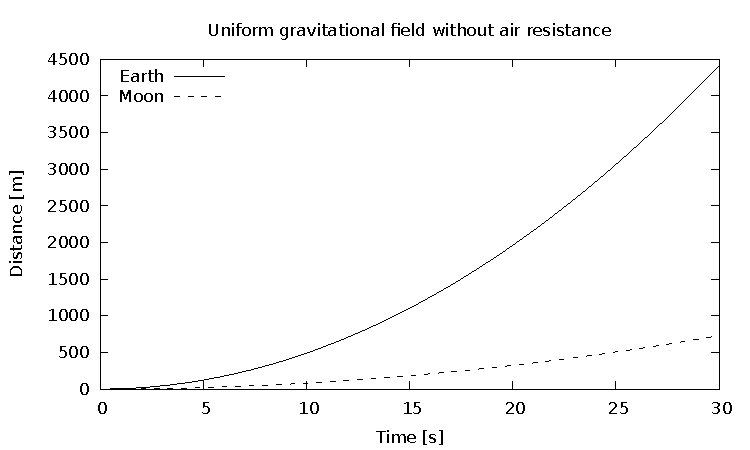
\includegraphics{gnuplot-bw}
% 	\caption{Černobílá varianta obrázku generovaného programem Gnuplot}\label{fig:gnuplot-bw}
% \end{figure}
% 
% \begin{figure}\centering
% 	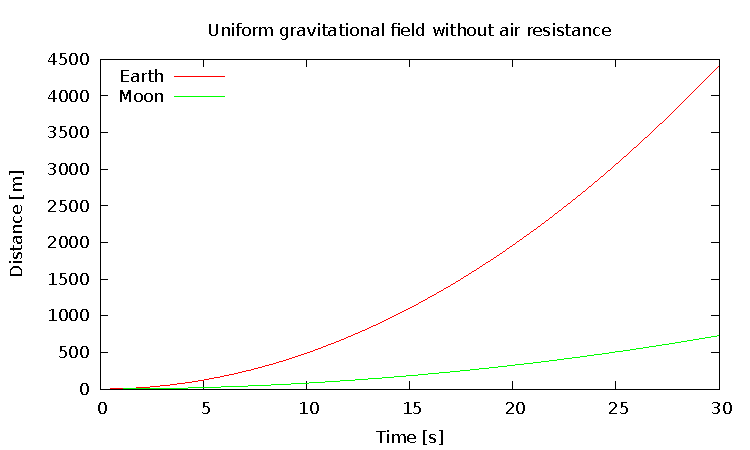
\includegraphics{gnuplot-col}
% 	\caption{Barevná varianta obrázku generovaného programem Gnuplot}\label{fig:gnuplot-col}
% \end{figure}
% 
% 
% \subsection{Tabulky}
% 
% Tabulky lze zadávat různě, např. v~prostředí \verb|tabular|, avšak pro jejich vkládání platí to samé, co pro obrázky -- použijte plovoucí prostředí, v~tomto případě \verb|table|. Například tabulka \ref{tab:matematika} byla vložena tímto způsobem.
% 
% \begin{table}\centering
% 	\caption[Příklad tabulky]{Zadávání matematiky}\label{tab:matematika}
% 	\begin{tabular}{|l|l|c|c|}\hline
% 		Typ		& Prostředí		& \LaTeX{}ovská zkratka	& \TeX{}ovská zkratka	\tabularnewline \hline \hline
% 		Text		& \verb|math|		& \verb|\(...\)|	& \verb|$...$|		\tabularnewline \hline
% 		Displayed	& \verb|displaymath|	& \verb|\[...\]|	& \verb|$$...$$|	\tabularnewline \hline
% 	\end{tabular}
% \end{table}
% 
% % % % % % % % % % % % % % % % % % % % % % % % % % % % 

\chapter{Obsah přiloženého CD}

%upravte podle skutecnosti

\begin{figure}
	\dirtree{%
		.1 readme.txt\DTcomment{stručný popis obsahu CD}.
		.1 exe\DTcomment{adresář se spustitelnou formou implementace}.
		.1 src.
		.2 impl\DTcomment{zdrojové kódy implementace}.
		.2 thesis\DTcomment{zdrojová forma práce ve formátu \LaTeX{}}.
		.1 text\DTcomment{text práce}.
		.2 thesis.pdf\DTcomment{text práce ve formátu PDF}.
		.2 thesis.ps\DTcomment{text práce ve formátu PS}.
	}
\end{figure}

\end{document}
